\usetikzlibrary{arrows,arrows.spaced,arrows.meta,decorations.markings,calc}

\newcommand{\xin}{\mathbf{x}_{\texttt{in}}}
\newcommand{\xout}{\mathbf{x}_{\texttt{out}}}
\newcommand{\xint}{\mathbf{x}_{\texttt{in}_t}}
\newcommand{\xoutt}{\mathbf{x}_{\texttt{out}_t}}
\newcommand{\localgrad}{\mathbf{L}}
\newcommand{\costgrad}{\mathbf{g}}

\definecolor{param_color}{rgb}{0.2, 0.6, 1.0}
\definecolor{comp_graph_node_bcolor}{rgb}{0.95,0.84,0.62}
\definecolor{comp_graph_loss_node_bcolor}{rgb}{0.93,0.43,0.34}
\definecolor{comp_graph_data_bcolor}{rgb}{1,1,1}
\definecolor{comp_graph_param_bcolor}{rgb}{0.97,0.88,0.35}
\definecolor{gray_neuron}{rgb}{0.7,0.7,0.7}
\definecolor{shared_term_color}{rgb}{0.85,0.8,1.0}
\definecolor{forwardpropcolor}{rgb}{0.2,0.9,0.2}
\definecolor{backwardpropcolor}{rgb}{0.9,0.2,0.2}
\definecolor{backwardpropcolor_params}{rgb}{0.97,0.88,0.35}

\newcommand{\highlight}[2][yellow]{\mathchoice%
  {\colorbox{#1}{$\displaystyle#2$}}%
  {\colorbox{#1}{$\textstyle#2$}}%
  {\colorbox{#1}{$\scriptstyle#2$}}%
  {\colorbox{#1}{$\scriptscriptstyle#2$}}}%

\tikzset{
  comp_graph_edge/.style={
        -Triangle
    }
}
\tikzset{
  comp_graph_edge_forward/.style={
        -Triangle,
        color=forwardpropcolor
    }
}
\tikzset{
  comp_graph_edge_backward/.style={
        -Triangle,
        color=backwardpropcolor
    }
}
\tikzset{
  comp_graph_edge_backward_params/.style={
        -Triangle,
        color=backwardpropcolor_params
    }
}
  
% https://tex.stackexchange.com/questions/27279/how-to-make-an-arrow-bigger-and-change-its-color-in-tikz/27287#27287
\tikzset{
  nn_edge/.style={
    decoration={markings,mark=at position 1 with {\arrow[scale=0.9]{spaced latex}}},
    postaction={decorate},
    shorten >=3.0pt
}}

\chapter{Backpropagation}\label{chapter:backpropagation}

\reviewcomment{Undergoing major revision.}

A key idea of neural nets is to decompose computation into a series of ``layers". In this chapter we will think of layers as modular blocks that can be chained together into a \textbf{computation graph}. Here's the computation graph for the two-layer MLP from Chapter $\ref{chapter:neural_nets}$:

\begin{figure}[h]
\begin{minipage}{.23\textwidth}
\centering
\begin{tikzpicture}[>=spaced latex]
\draw [thick] (0,-0.75) circle [radius=0.2] node[label={$\mathbf{x}$}] at (0,0.85);
\draw [thick] (0,0.1) node {$\vdots$};
\draw [thick] (0,0.75) circle [radius=0.2];

\draw [thick,dotted] (0.33,-1.2)  .. controls (0.43,-1.05) .. (0.43,-0.9);
\draw (0.4,-1.45) node {$\mathbf{W}_1$};

\draw [thick] [nn_edge] (0.2,-0.75) -- (0.8,-0.1);
\draw [thick] [nn_edge] (0.2,-0.75) -- (0.8,-0.75);
\draw [thick] [nn_edge] (0.2,-0.75) -- (0.8,0.75);
\draw [thick] [nn_edge] (0.2,-0.1) -- (0.8,-0.75);
\draw [thick] [nn_edge] (0.2,0.0) -- (0.8,0.0);
\draw [thick] [nn_edge] (0.2,0.1) -- (0.8,0.75);
\draw [thick] [nn_edge] (0.2,0.75) -- (0.8,0.75);
\draw [thick] [nn_edge] (0.2,0.75) -- (0.8,-0.75);
\draw [thick] [nn_edge] (0.2,0.75) -- (0.8,0.1);
\draw [thick, fill=gray_neuron] (1,0.75) circle [radius=0.2]  node[label={$\mathbf{z}$}] at (1.0,0.85);
\draw [thick] (1,0.1) node {$\vdots$};
\draw [thick, fill=gray_neuron] (1,-0.75) circle [radius=0.2];
\draw [thick] [nn_edge] (1.2,0.75) -- (1.8,0.75);
\draw [thick] [nn_edge] (1.2,0.0) -- (1.8,0.0);
\draw [thick] [nn_edge] (1.2,-0.75) -- (1.8,-0.75);
\draw [thick, fill=gray_neuron] (1,0.75) circle [radius=0.2]  node[label={$\mathbf{h}$}] at (2.0,0.85);
\draw [thick, fill=gray_neuron] (2.0,0.75) circle [radius=0.2];
\draw [thick] (2.0,0.1) node {$\vdots$};
\draw [thick, fill=gray_neuron] (2.0,-0.75) circle [radius=0.2];

\draw [thick,dotted] (2.33,-1.2)  .. controls (2.43,-1.05) .. (2.43,-0.9);
\draw (2.4,-1.45) node {$\mathbf{W}_2$};

\draw [thick] [nn_edge] (2.2,-0.75) -- (2.8,-0.75);
\draw [thick] [nn_edge] (2.2,-0.75) -- (2.8,0.75);
\draw [thick] [nn_edge] (2.2,-0.75) -- (2.8,0.0);
\draw [thick] [nn_edge] (2.2,-0.1) -- (2.8,-0.75);
\draw [thick] [nn_edge] (2.2,0.0) -- (2.8,0.0);
\draw [thick] [nn_edge] (2.2,0.1) -- (2.8,0.75);
\draw [thick] [nn_edge] (2.2,0.75) -- (2.8,0.75);
\draw [thick] [nn_edge] (2.2,0.75) -- (2.8,-0.75);
\draw [thick] [nn_edge] (2.2,0.75) -- (2.8,0.0);
\draw [thick] (3.0,-0.75) circle [radius=0.2] node[label={$\mathbf{y}$}] at (3.0,0.8);
\draw [thick] (3.0,0.1)  node {$\vdots$};
\draw [thick] (3.0,0.75) circle [radius=0.2];
\end{tikzpicture}
\end{minipage}
%
%
\begin{minipage}{0.77\textwidth}
\centering
\def\layerwidth{1.3}
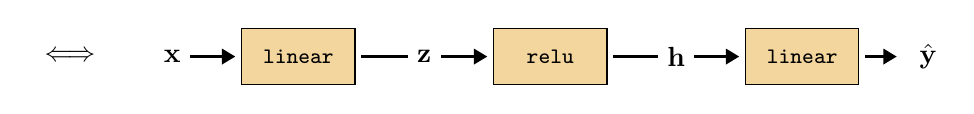
\begin{tikzpicture}[
cblock/.style={
draw,
fill=comp_graph_node_bcolor,
rectangle, 
inner sep=1.5mm,
minimum width=\layerwidth*0.9 cm,
minimum height=\layerwidth*0.5*0.9 cm,
font=\footnotesize}]
%
\draw [thick] [comp_graph_edge] (\layerwidth*0.5,0) -- (\layerwidth,0);
%\draw (0,0) rectangle ++(1,1);
\draw (\layerwidth*1.5,0) node [cblock] {\texttt{linear}};
\draw [thick] [comp_graph_edge] (\layerwidth*2,0) -- (\layerwidth*3,0);
\draw (\layerwidth*3.5,0) node [cblock] {\texttt{relu}};
\draw [thick] [comp_graph_edge] (\layerwidth*4,0) -- (\layerwidth*5,0);
\draw (\layerwidth*5.5,0) node [cblock] {\texttt{linear}};
\draw [thick] [comp_graph_edge] (\layerwidth*6,0) -- (\layerwidth*6.25,0);

\draw (\layerwidth*0.5,0) node [fill=comp_graph_data_bcolor] {$\mathbf{x}$};
\draw (\layerwidth*2.5,0) node [fill=comp_graph_data_bcolor] {$\mathbf{z}$};
\draw (\layerwidth*4.5,0) node [fill=comp_graph_data_bcolor] {$\mathbf{h}$};
\draw (\layerwidth*6.5,0) node [fill=comp_graph_data_bcolor] {$\hat{\mathbf{y}}$};

\draw (-0.5,0) node {$\iff$};
\end{tikzpicture}
\end{minipage}
\marginnote{\caption{}\label{fig:backpropagation:simple_MLP}}[-2.6cm]
\end{figure}


Each \colorbox{comp_graph_node_bcolor}{layer} takes in some inputs and transforms them into some outputs. We call this the $\texttt{forward}$ pass through the layer. If the layer has parameters, we will consider the parameters to be an \textit{input} to a parameter-free transformation:
\begin{align}
    \xout &= f(\xin,\theta)
\end{align}
Graphically, we will depict the forward operation of a layer like this:
\begin{figure}[h]
\centering
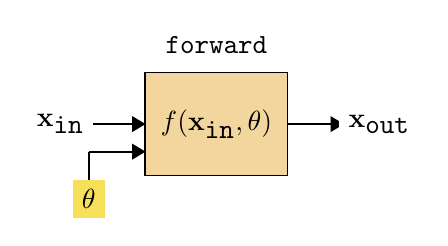
\begin{tikzpicture}%[>=spaced latex]
%
\def\layerwidth{1.8}
%
\draw [thick] [comp_graph_edge] (\layerwidth*0.6,-0.35) -- (\layerwidth,-0.35);
\draw [thick] (\layerwidth*0.6,-0.75) -- (\layerwidth*0.6,-0.35);
\draw [thick] [comp_graph_edge] (\layerwidth*0.5,0) -- (\layerwidth,0);
\draw (\layerwidth*1.5,0) node [fill=comp_graph_node_bcolor,draw, inner sep=2mm, minimum height=1.3cm] {$f(\xin, \theta)$};
\draw [thick] [comp_graph_edge] (\layerwidth*2,0) -- (\layerwidth*2.4,0);
%
\draw (\layerwidth*0.6,-0.95) node [fill=comp_graph_param_bcolor] {$\theta$};
\draw (\layerwidth*0.4,0) node [fill=comp_graph_data_bcolor] {$\xin$};
\draw (\layerwidth*2.65,0) node [fill=comp_graph_data_bcolor] {$\xout$};
\draw (\layerwidth*1.5,1) node {\texttt{forward}};
%
\end{tikzpicture}
\label{fig:backpropagation:mod_block_forward}
\end{figure}

% \begin{figure}[h]
% \centering
% \begin{tikzpicture}%[>=spaced latex]
% %
% \def\layerheight{1.0}

% \draw [thick] [comp_graph_edge] (0,0) -- (0,\layerheight);
% %\draw (0,0) rectangle ++(1,1);
% \draw (0,\layerheight*1.5) node [fill=comp_graph_node_bcolor,draw, inner sep=2mm] {$f(\xin)$};
% \draw [thick] [comp_graph_edge] (0,\layerheight*2) -- (0,\layerheight*3);

% \draw (0,\layerheight*0.4) node [fill=comp_graph_data_bcolor] {$\xin$};
% \draw (0,\layerheight*2.4) node [fill=comp_graph_data_bcolor] {$\xout$};

% \end{tikzpicture}
% \label{fig:backpropagation:mod_block}
% \end{figure}

% \begin{figure}[h]
%     \centering
%     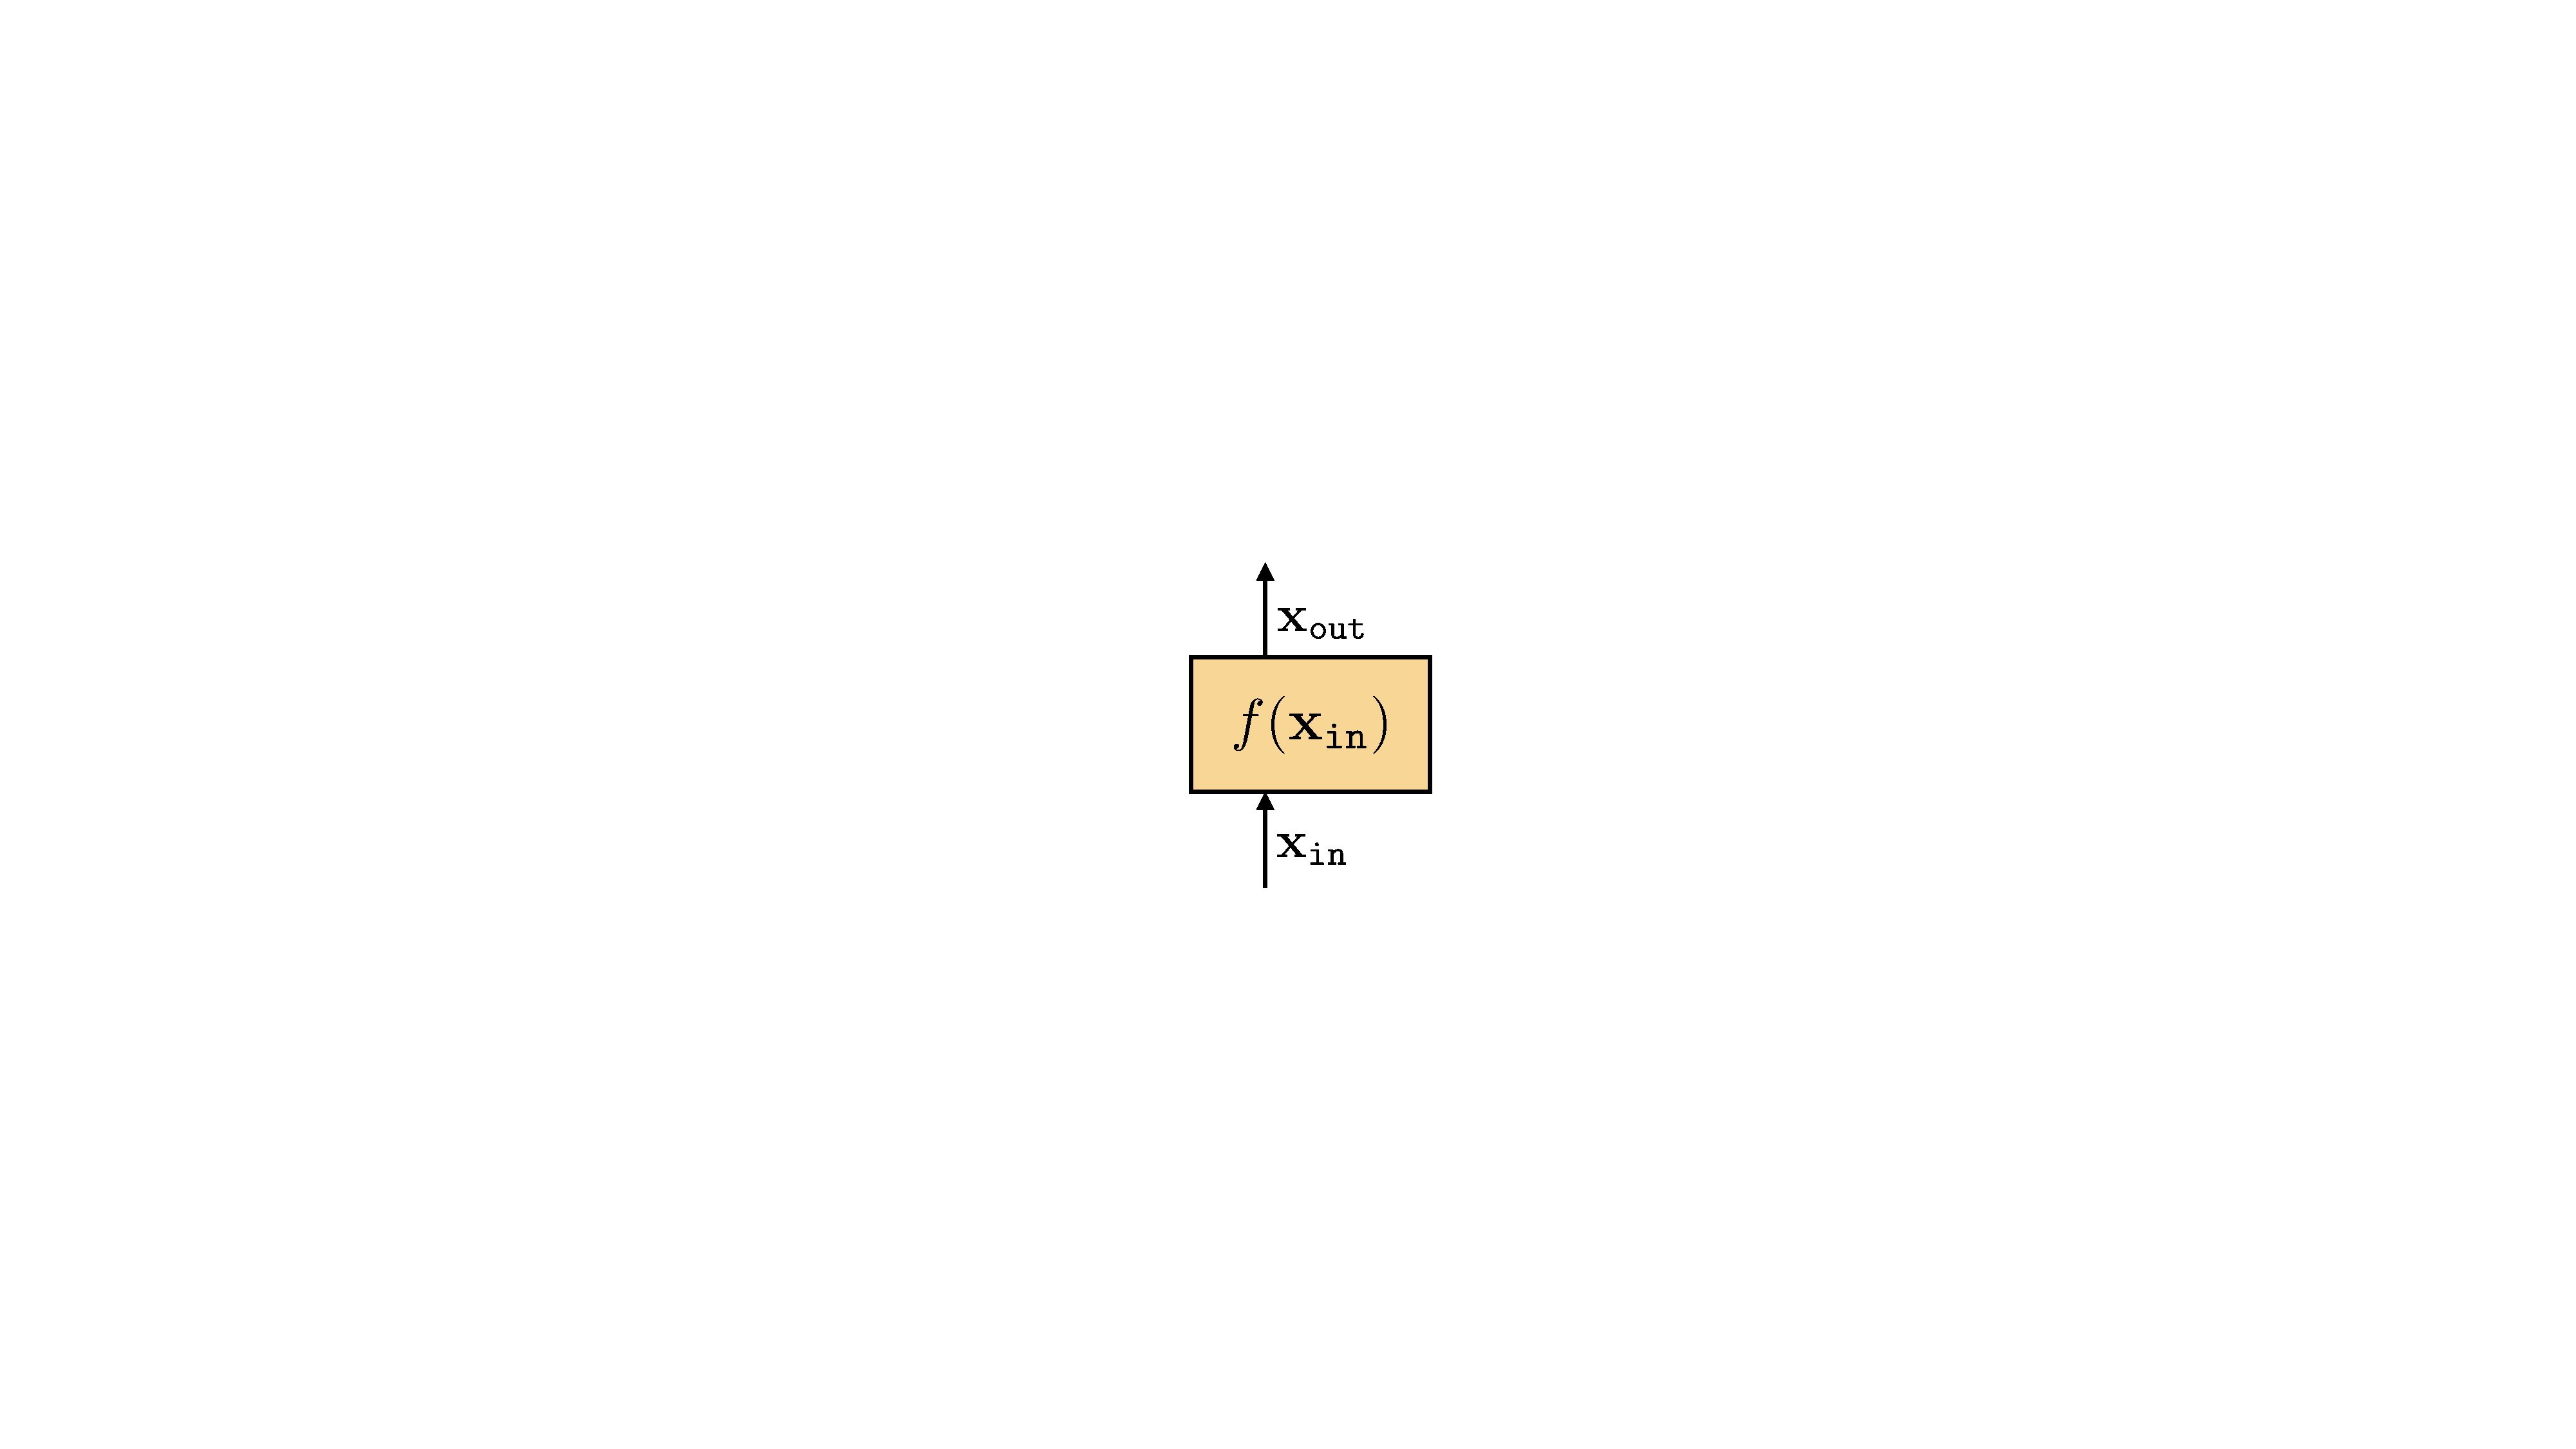
\includegraphics[width=0.18\linewidth]{./figures/backpropagation/mod_block.pdf}
%     \label{fig:mod_block}
% \end{figure}

%A graph of computational blocks like this is called a \textbf{computation graph}.

The learning problem is to find the parameters \colorbox{comp_graph_param_bcolor}{$\theta$} that achieve a desired mapping. Usually we will solve this problem via gradient descent. The question of this chapter is: how do we compute the gradients? 

\textbf{Backpropagation} is an algorithm that efficiently calculates the gradient of the loss w.r.t. each and every parameter in a computation graph. It relies on a special new operation, called \texttt{backward} that, just like \texttt{forward}, can be defined for each layer, and acts in isolation from the rest of the graph. But first, before we get to defining \texttt{backward}, we will build up some intuition about the key trick backprop will exploit.

\section{The trick of backprop: reuse of computation}

To start, we will consider a simple computation graph that is a chain of functions $f_L \circ f_{L-1} \circ \cdots f_2 \circ f_1$, with each function $f_l$ parameterized by $\theta_l$.\marginnote{Such a computation graph could represent an MLP, for example, which we will see in the next section.}[-0.4cm] We aim to optimize the parameterize w.r.t. a loss function $\mathcal{L}$. The loss can be treated as another node in our computation graph, which takes in $\mathbf{x}_L$ (the output of $f_L$) and outputs a scalar $J$, the loss. This computation graph looks as follows:
\begin{figure}
    \centering
    \def\layerwidth{1.4}
    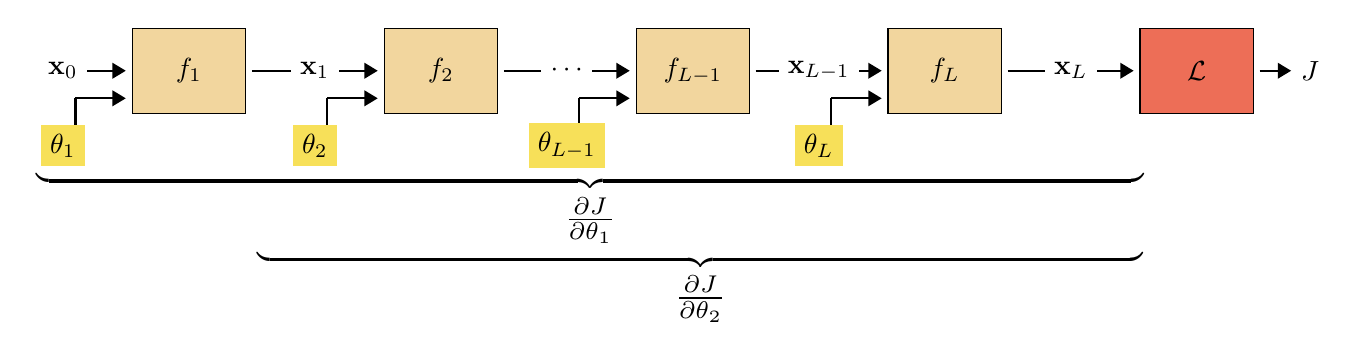
\begin{tikzpicture}[
    cblock/.style={
    draw,
    fill=comp_graph_node_bcolor,
    rectangle, 
    inner sep=1.5mm,
    minimum width=\layerwidth*0.9 cm,
    minimum height=\layerwidth*0.75*0.9 cm}]
    %
    %
    % draw f nodes
    \def\fnames {{"$f_0$","$f_1$","$f_2$","$f_{L-1}$","$f_L$"}}
    \foreach \x in {1,2,3,4} {
        \pgfmathparse{\fnames[\x]};
        \draw ($(\layerwidth*2*\x-\layerwidth+\layerwidth*0.5,0)$) node [cblock] {\pgfmathresult};
    }
    % draw data arrows
    \draw [thick] [comp_graph_edge] (\layerwidth*0.5,0) -- (\layerwidth,0);
    \foreach \x in {1,2,3,4} {
        % data arrow
        \draw [thick] [comp_graph_edge] (\layerwidth*2*\x,0) -- (\layerwidth*2*\x+\layerwidth,0);
    }
    \draw [thick] [comp_graph_edge] (\layerwidth*10,0) -- (\layerwidth*10.25,0);
    %
    % draw param arrows
    \foreach \x in {0,1,2,3} {
        \draw [thick] [comp_graph_edge] (\layerwidth*2*\x+\layerwidth*0.6,-0.35) -- (\layerwidth*2*\x+\layerwidth,-0.35);
        \draw [thick] (\layerwidth*2*\x+\layerwidth*0.6,-0.75) -- (\layerwidth*2*\x+\layerwidth*0.6,-0.35);
    }
    %
    % draw data and params
    \def\datanames {{"$\mathbf{x}_0$","$\mathbf{x}_1$","$\cdots$","$\mathbf{x}_{L-1}$","$\mathbf{x}_L$"}}
    \def\paramnames {{"$\theta_1$","$\theta_2$","$\theta_{L-1}$","$\theta_{L}$"}}
    \foreach \x in {0,1,2,3,4} {
        \pgfmathparse{\datanames[\x]};
        \draw ($(\layerwidth*2*\x+\layerwidth*0.5,0)$) node [fill=comp_graph_data_bcolor] {\pgfmathresult};
        %
    };
    \foreach \x in {0,1,2,3} {
        \pgfmathparse{\paramnames[\x]};
        \draw ($(\layerwidth*2*\x+\layerwidth*0.5,-0.95)$) node [fill=comp_graph_param_bcolor] {\pgfmathresult};
    };
    %
    % loss node
    \draw (\layerwidth*9.5,0) node [cblock, fill=comp_graph_loss_node_bcolor] {$\mathcal{L}$};
    \draw (\layerwidth*10.4,0) node [fill=comp_graph_data_bcolor] {$J$};
    %
    \draw (7.5,-1.4) node {$\underbrace{\quad\quad\quad\quad\quad\quad\quad\quad\quad\quad\quad\quad\quad\quad\quad\quad\quad\quad\quad\quad\quad\quad\quad\quad\quad\quad\quad\quad\quad\quad\quad\quad\quad\quad\quad\quad\quad\quad\quad\quad}$};
    \draw (7.5,-1.9) node [scale=1.25] {$\frac{\partial J}{\partial \theta_1}$};
    \draw (8.9,-2.4) node {$\underbrace{\quad\quad\quad\quad\quad\quad\quad\quad\quad\quad\quad\quad\quad\quad\quad\quad\quad\quad\quad\quad\quad\quad\quad\quad\quad\quad\quad\quad\quad\quad\quad\quad}$};
    \draw (8.9,-2.9) node [scale=1.25] {$\frac{\partial J}{\partial \theta_2}$};
    %
    \end{tikzpicture}
    \vspace{-1cm}
    \label{fig:backpropagation:composed_modules}
\end{figure}
\marginnote{This computation graph is a narrow tree; the parameters live on branches of length 1. This can be easier to see when we plot it with data and parameters as nodes and edges as the functions:
\medbreak
    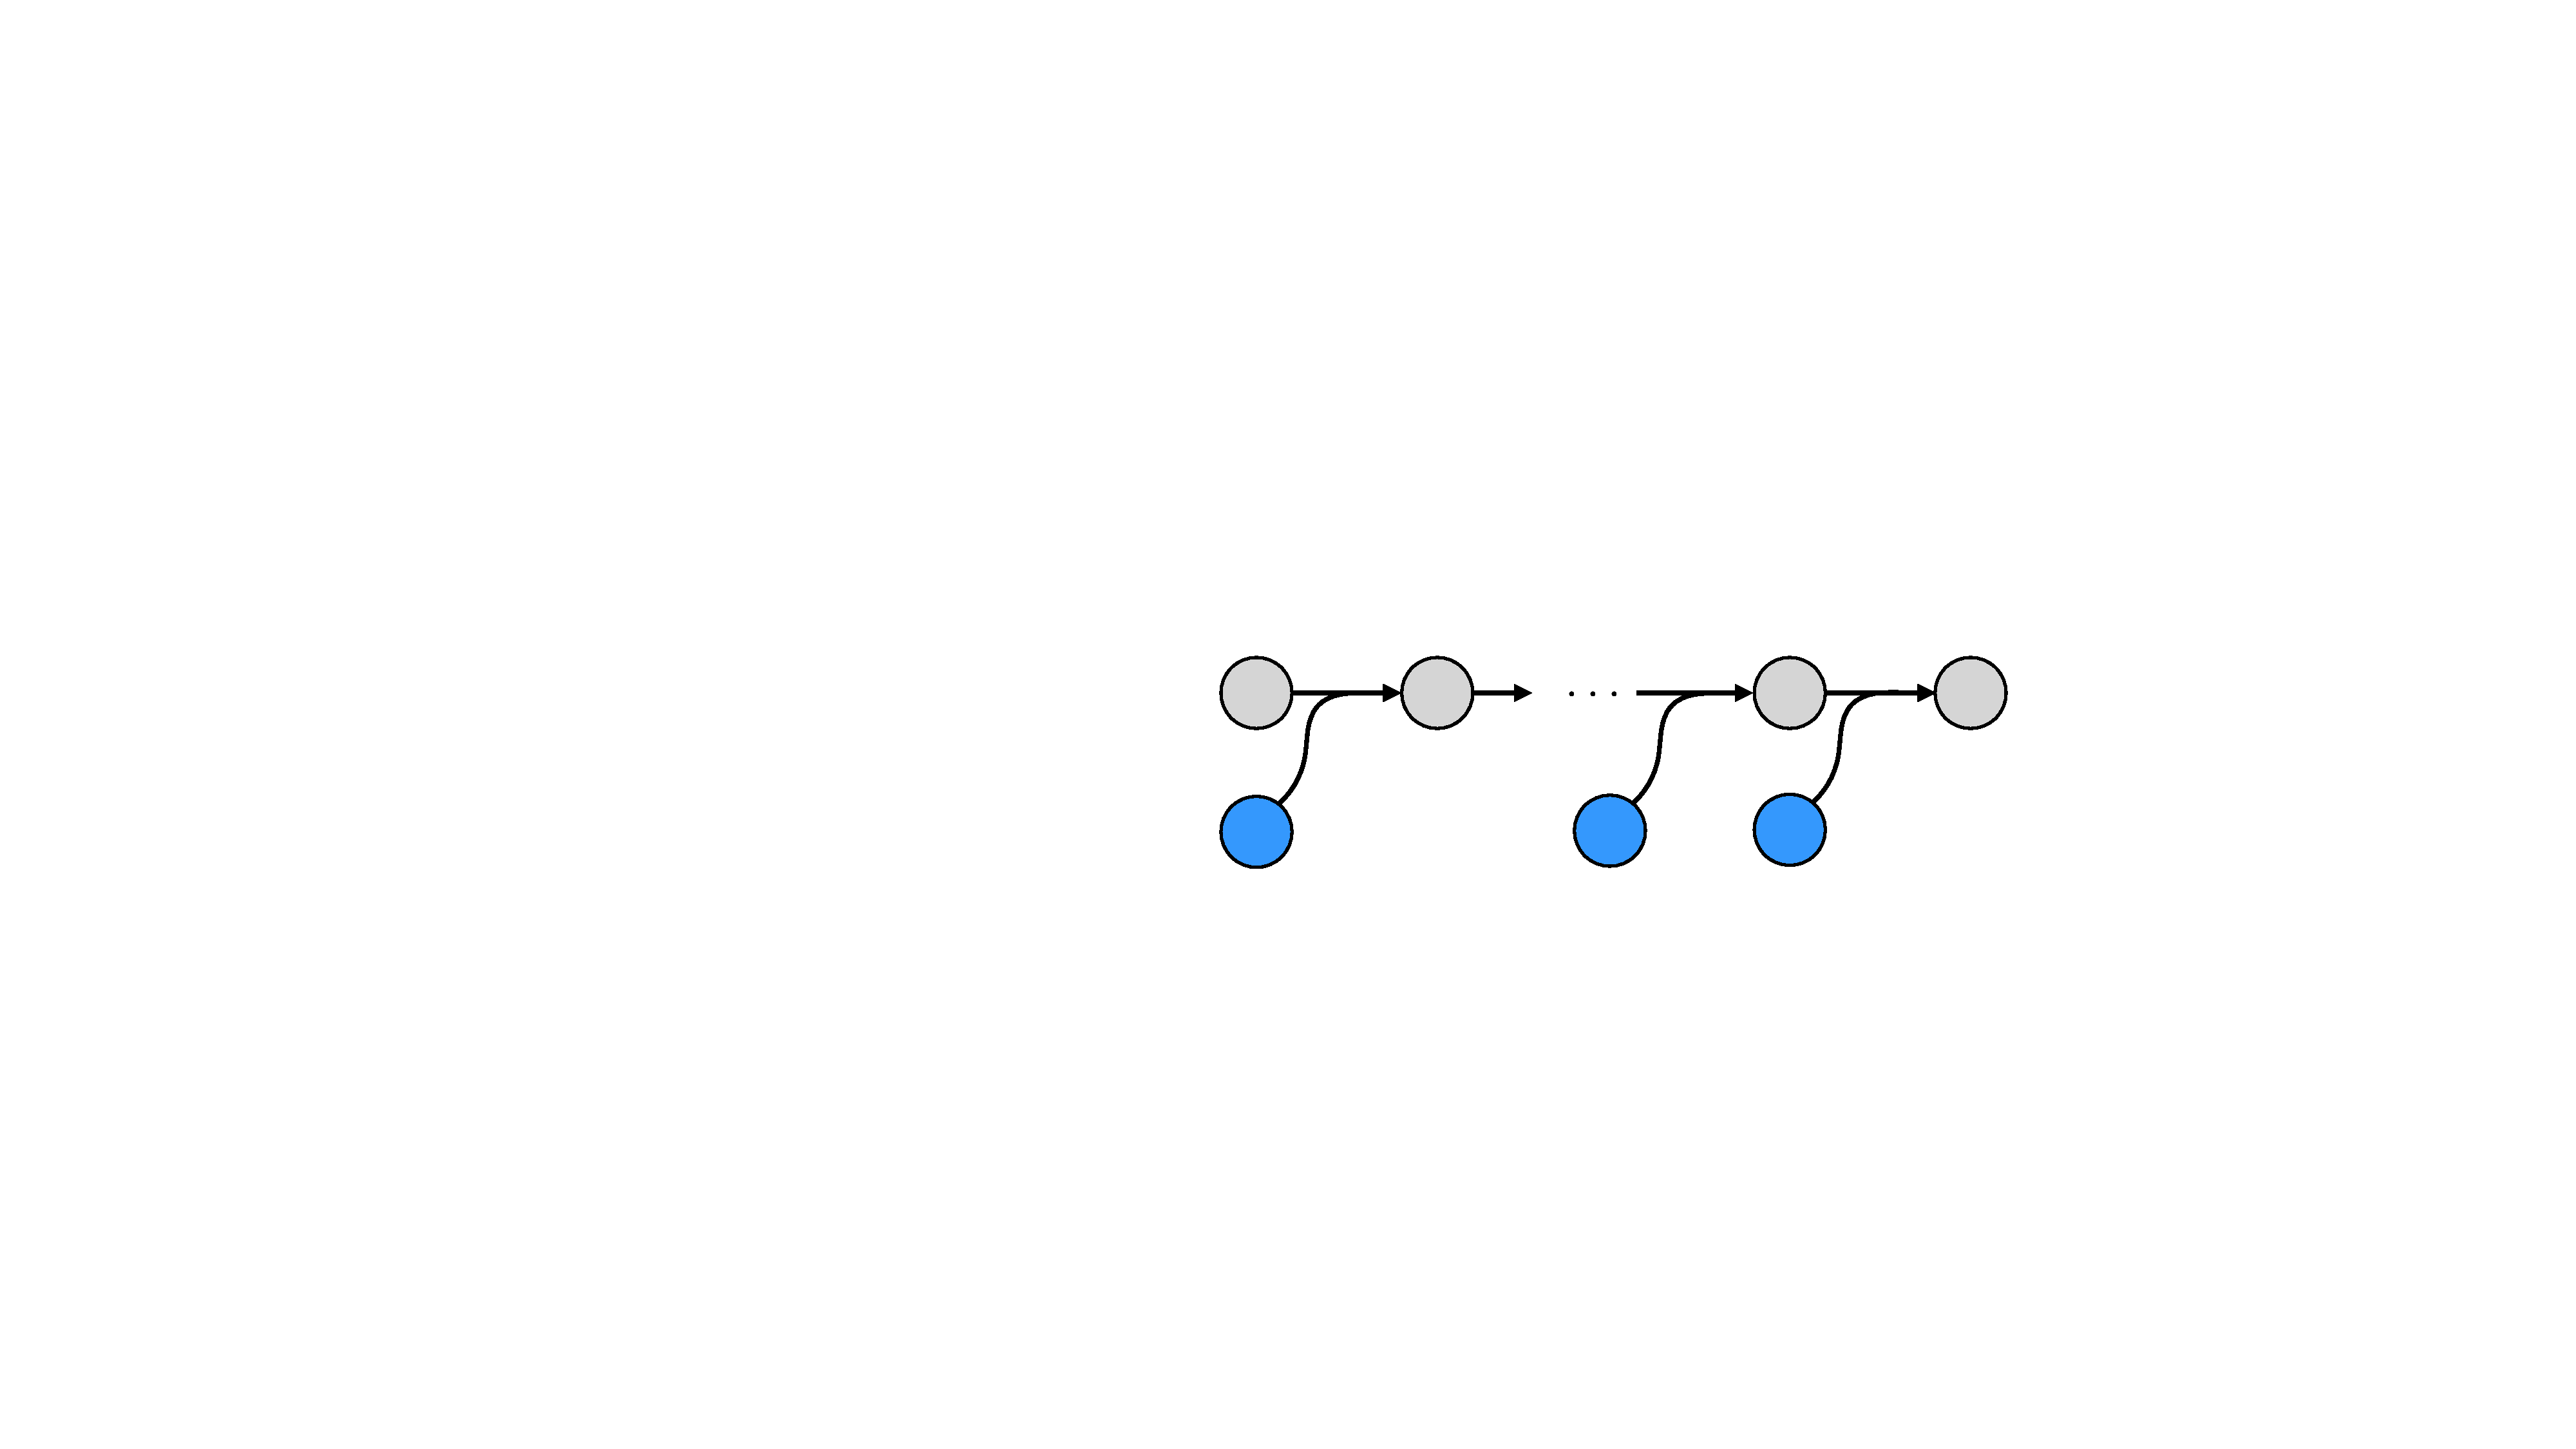
\includegraphics[width=0.9\linewidth]{./figures/backpropagation/cgraph_tree.pdf}
}[-4cm]

Our goal is to update all the values highlighted in yellow: $\theta_1$, $\theta_2$ and so forth. To do so we need to compute the gradients $\frac{\partial J}{\partial \theta_1}$, $\frac{\partial J}{\partial \theta_2}$, etc. Each of these gradients can be calculated via the chain rule. Here is the chain rule written out for the gradients for $\theta_1$ and $\theta_2$:
\begin{align}
    \frac{\partial J}{\partial \theta_1} &= \highlight[shared_term_color]{\frac{\partial J}{\partial \mathbf{x}_L}\frac{\partial \mathbf{x}_L}{\partial \mathbf{x}_{L-1}} \cdots \frac{\partial \mathbf{x}_3}{\partial \mathbf{x}_2}} \frac{\partial \mathbf{x}_2}{\mathbf{x}_1}\frac{\partial \mathbf{x}_1}{\partial \mathbf{\theta}_1}\\
    \frac{\partial J}{\partial \theta_2} &=  \highlight[shared_term_color]{\frac{\partial J}{\partial \mathbf{x}_{L}}\frac{\partial \mathbf{x}_L}{\partial \mathbf{x}_{L-1}} \cdots \frac{\partial \mathbf{x}_3}{\partial \mathbf{x}_2}} \frac{\partial \mathbf{x}_2}{\partial \theta_2}
\end{align}
Rather than evaluating both equations separately, we notice that all the terms highlighted in blue are shared. We only need to evaluate this product once, and then can use it to compute both $\frac{\partial J}{\partial \theta_1}$ and $\frac{\partial J}{\partial \theta_2}$. Now notice that this pattern of reuse can be applied in the same way for $\theta_3$, $\theta_4$, and so on. This is the whole trick of backpropagation: rather than computing each layer's gradients independently, observe that they share many of the same terms, so we might as well calculate each shared term once and reuse them. \marginnote{This strategy, in general, is called {\bf dynamic programming}.}[-0.6cm]

\section{\texttt{Backward} for a generic layer}
To come up with a general algorithm for reusing all the shared computation, we will first look at one generic layer in isolation, and see what we need in order to update its parameters.
\begin{figure}[h]
\centering
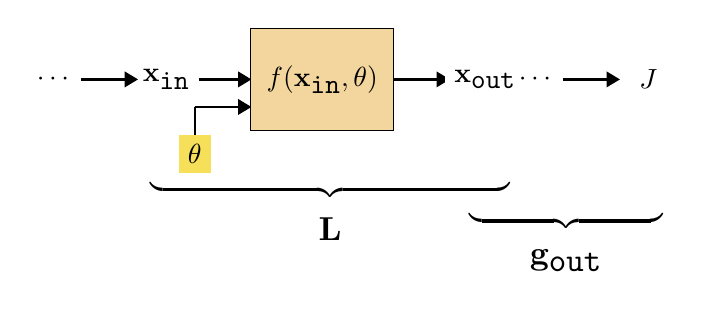
\begin{tikzpicture}%[>=spaced latex]
%
\def\layerwidth{1.8}
%
\draw [thick] [comp_graph_edge] (\layerwidth*0.6,-0.35) -- (\layerwidth,-0.35);
\draw [thick] (\layerwidth*0.6,-0.75) -- (\layerwidth*0.6,-0.35);
\draw [thick] [comp_graph_edge] (\layerwidth*0.5,0) -- (\layerwidth,0);
\draw (\layerwidth*1.5,0) node [fill=comp_graph_node_bcolor,draw, inner sep=2mm, minimum height=1.3cm] {$f(\xin, \theta)$};
\draw [thick] [comp_graph_edge] (\layerwidth*2,0) -- (\layerwidth*2.4,0);
%
\draw (\layerwidth*0.6,-0.95) node [fill=comp_graph_param_bcolor] {$\theta$};
\draw (\layerwidth*0.4,0) node [fill=comp_graph_data_bcolor] {$\xin$};
\draw (\layerwidth*2.65,0) node [fill=comp_graph_data_bcolor] {$\xout$};
\draw (\layerwidth*3,0) node {$\cdots$};
\draw [thick] [comp_graph_edge] (\layerwidth*3.2,0) -- (\layerwidth*3.6,0);
\draw (\layerwidth*3.8,0) node {$J$};
\draw [thick] [comp_graph_edge] (-0.2*\layerwidth,0) -- (0.2*\layerwidth,0);
\draw (-0.4*\layerwidth,0) node {$\cdots$};
%
\draw (2.8,-1.4) node {$\underbrace{\quad\quad\quad\quad\quad\quad\quad\quad\quad\quad\quad\quad\quad}$};
\draw (2.8,-1.9) node [scale=1.2] {$\localgrad$};
\draw (5.8,-1.8) node {$\underbrace{\quad\quad\quad\quad\quad\quad\quad}$};
\draw (5.8,-2.3) node [scale=1.2] {$\costgrad_\texttt{out}$};
%
\end{tikzpicture}
\end{figure}
\marginnote{The braces represent the part of the computation graph we need to consider in order to evaluate $\localgrad$ and $\costgrad$}[-0.0cm]

Here we have introduced two new shorthands, $\localgrad$ and $\costgrad$ -- these represent arrays of partial derivatives, defined below, and they are the key arrays we need to keep track of to do backprop. They are defined as:
%To update $\theta$ for this layer, we just need to know $\frac{\partial J}{\partial \theta}$
%This strategy involves two key matrices: 1) the vector of derivatives of the cost $J$ w.r.t to each layer's inputs, and 2) the matrix of derivatives of the outputs of each layer with respect to its inputs. We define shorthand for these below:
\marginnote{All these arrays represent the gradient \textit{at a single operating point} --  that of the current value of the data and parameters.}[1cm]
\begin{align}
    \costgrad &\triangleq \frac{\partial J}{\partial [\xin, \xout, \theta]} &&\quad\quad \triangleleft \quad \text{grad of cost}\\
     &\quad\quad \costgrad^{\xin} \triangleq \frac{\partial J}{\partial \xin} &&\quad\quad \triangleleft \quad \text{... w.r.t. layer inputs} \quad [1 \times |\xin|]\\
     &\quad\quad \costgrad^{\xout} \triangleq \frac{\partial J}{\partial \xout} &&\quad\quad \triangleleft \quad \text{... w.r.t. layer outputs} \quad [1 \times |\xout|]\\
     &\quad\quad \costgrad^{\theta} \triangleq \frac{\partial J}{\partial \theta} &&\quad\quad \triangleleft \quad \text{... w.r.t. layer params} \quad [1 \times |\theta|]\\
    \localgrad &\triangleq \frac{\partial \xout}{\partial [\xin, \theta]} &&\quad\quad \triangleleft \quad \text{grad of layer}\\
    &\quad\quad \localgrad^{\mathbf{x}} \triangleq \frac{\partial \xout}{\partial \xin} &&\quad\quad \triangleleft \quad \text{... w.r.t. layer input data} \quad [|\xout| \times |\xin|]\\
    &\quad\quad \localgrad^{\theta} \triangleq \frac{\partial \xout}{\partial \theta} &&\quad\quad \triangleleft \quad \text{... w.r.t. layer params} \quad [|\xout| \times |\theta|]
    %\mathbf{F}_l &\triangleq \frac{\partial \mathbf{x}_{l}}{\partial \mathbf{x}_{l-1}} = \frac{\partial f_l(\mathbf{x}_{l-1})}{\partial \mathbf{x}_{l-1}} &\quad\quad \triangleleft \quad [N \times M]
\end{align}

These arrays give a simple formula for computing the gradient we need -- $\frac{\partial J}{\partial \theta}$ -- in order to \texttt{update} $\theta$ to minimize the cost:
%\begin{align}
%    \frac{\partial J}{\partial \theta_l} = \costgrad_l\localgrad^{\theta}_l \quad\quad \triangleleft \quad [1 \times |\xout|]\cdot[|\xout| \times |\theta|] \rightarrow [1 \times \theta]] \label{eqn:backpropagation:param_update}
%\end{align}
\begin{align}
    \frac{\partial J}{\partial \theta} &= \costgrad_{\texttt{out}}\localgrad^{\theta}\\
    \theta^{i+1} &\leftarrow \theta^{i} - \eta \Big(\frac{\partial J}{\partial \theta}\Big)^T &&\quad\quad \triangleleft \quad \texttt{update} \label{eqn:backpropagation:djdtheta}
\end{align}
\marginnote{The transpose is because, by convention $\theta$ is a column vector while $\frac{\partial J}{\partial \theta}$ is a row vector; see Appendix.}[-0.4cm]

The remaining question is just: how do we get $\costgrad_l$ and $\localgrad^{\theta}_l$ for layer $l$? 

Computing $\localgrad$ is an entirely local process: for each layer, we just need to know the functional form of its derivative, $f^{\prime}$, which we then evaluate at the operating point $[\xin, \theta]$ to obtain $\localgrad = f^{\prime}(\xin,\theta)$.

Computing $\costgrad$ is a bit trickier; it requires evaluating the chain rule, and depends on all the layers between $\xout$ and $J$. However, this can be computed iteratively: once we know $\costgrad_l$, computing $\costgrad_{l-1}$ is just one more matrix multiply! This can be summarized with the following recurrence relation:
\begin{align}
    \costgrad_{\texttt{in}} &= \costgrad_{\texttt{out}}\localgrad^{\mathbf{x}} &&\quad\quad \triangleleft \quad \text{``backpropagation of errors"} \label{eqn:backpropagation:backward}
\end{align}
This recurrence is is essence of backprop: it sends ``error signals" (gradients) backwards through the network, starting at the last layer and iteratively applying Equation \ref{eqn:backpropagation:backward} to
compute $\costgrad$ for each previous layer.
\marginnote{Deep learning libraries like Pytorch have a \texttt{.grad} field associated with each variable (data, activations, parameters). This field reprsents $\frac{\partial J}{\partial v}$ for each variable $v$.}[-0.4cm]

We are finally ready to define the full \texttt{backward} function promised at the beginning of this chapter! It consists of the following operation, which has three inputs -- $\xin, \theta, \costgrad_{\texttt{out}}$-- and two outputs -- $\costgrad_{\texttt{in}}$ and $\frac{\partial J}{\partial \theta}$:
\begin{figure}[h]
\centering
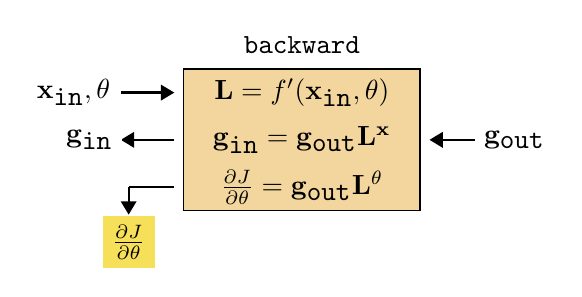
\begin{tikzpicture}%[>=spaced latex]
%
\def\layerwidth{1.8}
%
\draw [thick] [comp_graph_edge] (0.4,0.6) -- (\layerwidth*0.6,0.6);
\draw [thick] [comp_graph_edge] (\layerwidth*0.6,0) -- (0.4,0);
\draw [thick] [comp_graph_edge] (0.5,-0.6) -- (0.5,-0.95);
\draw [thick] (\layerwidth*0.6,-0.6) -- (0.5,-0.6);
\draw (\layerwidth*1.5,0) node [fill=comp_graph_node_bcolor,draw, inner sep=2mm, minimum height=1.8cm, minimum width=3.0cm] {};
\draw (\layerwidth*1.5,1.2) node {\texttt{backward}};
\draw (\layerwidth*1.5,0.6) node  {$\localgrad = f^{\prime}(\xin,\theta)$};
\draw (\layerwidth*1.5,0) node  {$\costgrad_{\texttt{in}} = \costgrad_{\texttt{out}}\localgrad^{\mathbf{x}}$};
\draw (\layerwidth*1.5,-0.6) node  {$\frac{\partial J}{\partial \theta} = \costgrad_{\texttt{out}}\localgrad^{\theta}$};
\draw [thick] [comp_graph_edge] (\layerwidth*2.8,0) -- (\layerwidth*2.4,0);
%
\draw (0.5,-1.3) node [fill=comp_graph_param_bcolor] {$\frac{\partial J}{\partial \theta}$};
\draw (-0.2,0.6) node [fill=comp_graph_data_bcolor] {$\xin, \theta$};
\draw (0,0) node [fill=comp_graph_data_bcolor] {$\costgrad_{\texttt{in}}$};
\draw (\layerwidth*3,0) node [fill=comp_graph_data_bcolor] {$\costgrad_{\texttt{out}}$};
%
\end{tikzpicture}
\label{fig:backpropagation:mod_block_backward}
\end{figure}

% For any $\frac{\partial J}{\partial \theta_l}$, we have:
% \begin{align}
%     \frac{\partial J}{\partial \theta_l} = \frac{\partial J}{\partial \mathbf{x}_l}\frac{\partial \mathbf{x}_l}{\partial \theta_l}
% \end{align}
% This says that all the parameter updates can be computed with just one further matrix multiply once we know $\frac{\partial J}{\partial \mathbf{x}_l}$ for all $l$. Now, the trick is to work backwards to compute all the $\frac{\partial J}{\partial \mathbf{x}_l}$, because:
% \begin{align}
%     \frac{\partial J}{\partial \mathbf{x}_l} = \frac{\partial J}{\partial \mathbf{x}_{l+1}}\frac{\partial \mathbf{x}_{l+1}}{\partial \mathbf{x}_l}
% \end{align}
% So, once we know $\frac{\partial J}{\partial \mathbf{x}_{l+1}}$ we can compute $\frac{\partial J}{\partial \mathbf{x}_{l}}$ with just one additional matrix multiply.

%The value of the blue terms is $\frac{\partial j}{\partial \mathbf{x}_2}$. Once we have calculated this value, we can 

%Indeed, once we've computed $\frac{\partial \mathbf{x}_{L}}{\partial \mathbf{x}_{l}}$, we can compute $\frac{\partial \mathbf{x}_{L}}{\partial \mathbf{x}_{l-1}}$ with just one more multiply:
%\begin{align}
%    \frac{\partial \mathbf{x}_{L}}{\partial \mathbf{x}_{l-1}} = \frac{\partial \mathbf{x}_{L}}{\partial \mathbf{x}_{l}} \frac{\partial \mathbf{x}_{l}}{\partial \mathbf{x}_{l-1}}
%\end{align}

%\section{Backprop through chains}


% \begin{align}
%     \xout &= f(\xin,\theta) &&\quad\quad \triangleleft \quad \texttt{forward}\\
%     \costgrad_{\texttt{in}} &= \costgrad_{\texttt{out}}\localgrad^{\mathbf{x}} &&\quad\quad \triangleleft \quad \texttt{backward}
% \end{align}

% And then update parameters:
% \begin{align}
%     \frac{\partial J}{\partial \theta} &= \costgrad_{\texttt{out}}\localgrad^{\theta} &&\quad\quad \triangleleft \quad \texttt{update}
% \end{align}


\section{The full algorithm: forward pass, then backward pass}
We are ready now to define the full backprop algorithm. In the last section we saw that we can easily compute the gradient update for $\theta_l$ once we have computed $\localgrad_l$ and $\costgrad_l$.\marginnote{$\costgrad_l$ and $\localgrad_l$ are the $\costgrad$ and $\localgrad$ arrays for layer $l$.}[-0.0cm]

So, we just need to order our operations so that when we get to updating layer $l$ we have these two arrays ready. The way to do it is to first compute a \textbf{forward pass} through the entire network, which means starting with input data $\mathbf{x}_0$ and evaluating layer by layer to produce the sequence $\mathbf{x}_0, \mathbf{x}_1, \ldots, \mathbf{x}_L$. Here is what the forward pass looks like:
\begin{figure}[h]
    \centering
    \def\layerwidth{1.4}
    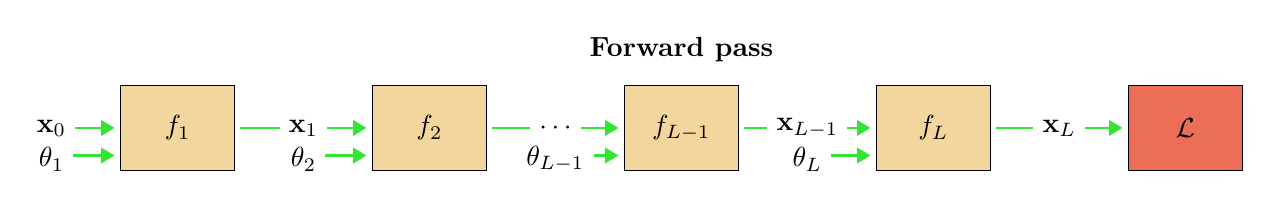
\begin{tikzpicture}[
    cblock/.style={
    draw,
    fill=comp_graph_node_bcolor,
    rectangle, 
    inner sep=1.5mm,
    minimum width=\layerwidth*0.9 cm,
    minimum height=\layerwidth*0.75*0.9 cm}]
    %
    %
    % draw f nodes
    \def\fnames {{"$f_0$","$f_1$","$f_2$","$f_{L-1}$","$f_L$"}}
    \foreach \x in {1,2,3,4} {
        \pgfmathparse{\fnames[\x]};
        \draw ($(\layerwidth*2*\x-\layerwidth+\layerwidth*0.5,0)$) node [cblock] {\pgfmathresult};
    }
    % draw data arrows
    \draw [thick] [comp_graph_edge_forward] (\layerwidth*0.5,0) -- (\layerwidth,0);
    \foreach \x in {1,2,3,4} {
        % data arrow
        \draw [thick] [comp_graph_edge_forward] (\layerwidth*2*\x,0) -- (\layerwidth*2*\x+\layerwidth,0);
    }
    %\draw [thick] [comp_graph_edge_forward] (\layerwidth*10,0) -- (\layerwidth*10.25,0);
    %
    % draw param arrows
    \foreach \x in {0,1,2,3} {
        \draw [thick] [comp_graph_edge_forward] (\layerwidth*2*\x+\layerwidth*0.6,-0.35) -- (\layerwidth*2*\x+\layerwidth,-0.35);
    }
    %
    % draw data and params
    \def\datanames {{"$\mathbf{x}_0$","$\mathbf{x}_1$","$\cdots$","$\mathbf{x}_{L-1}$","$\mathbf{x}_L$"}}
    \def\paramnames {{"$\theta_1$","$\theta_2$","$\theta_{L-1}$","$\theta_{L}$"}}
    \foreach \x in {0,1,2,3,4} {
        \pgfmathparse{\datanames[\x]};
        \draw ($(\layerwidth*2*\x+\layerwidth*0.5,0)$) node [fill=white] {\pgfmathresult};
        %
    };
    \foreach \x in {0,1,2,3} {
        \pgfmathparse{\paramnames[\x]};
        \draw ($(\layerwidth*2*\x+\layerwidth*0.5,-0.4)$) node [fill=white] {\pgfmathresult};
    };
    %
    % loss node
    \draw (\layerwidth*9.5,0) node [cblock, fill=comp_graph_loss_node_bcolor] {$\mathcal{L}$};
    %\draw (\layerwidth*10.4,0) node [fill=comp_graph_data_bcolor] {$J$};
    %
    \draw (\layerwidth*5.5,1.0) node {\textbf{Forward pass}};
    %
    \end{tikzpicture}
\end{figure}

%We need this sequence because, in general, $\localgrad$ for a layer will be a function of $\xin$ and $\theta$ for that layer -- so we need the full sequence of inputs and outputs to each layer to get compute the full sequence $\localgrad_1, \localgrad_2, \ldots$. 

Next, we compute a \textbf{backward pass}, iteratively evaluating the $\costgrad$'s and obtaining the sequence $\costgrad_L, \costgrad_{L-1}, \ldots$, as well as the parameter gradients for each layer: %Remember that to compute $\costgrad$ for a layer, we need $\localgrad$ for that layer, so on the
\marginnote{We needed to run the forward pass before the backward pass because $\texttt{backward}$ for each layer requires as input not just $\costgrad_{\texttt{out}}$ but also $\xin$, which we only will know, for each layer, after running the forward pass.}[-0.2cm]
\begin{figure}[h]
    \centering
    \def\layerwidth{1.4}
    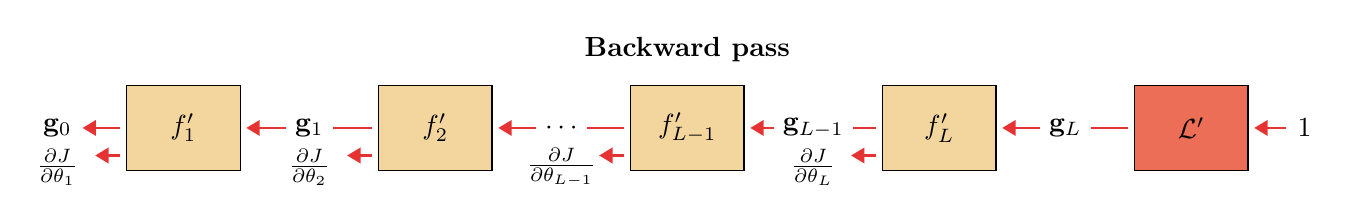
\begin{tikzpicture}[
    cblock/.style={
    draw,
    fill=comp_graph_node_bcolor,
    rectangle, 
    inner sep=1.5mm,
    minimum width=\layerwidth*0.9 cm,
    minimum height=\layerwidth*0.75*0.9 cm}]
    %
    %
    % draw f nodes
    \def\fnames {{"$f^{\prime}_0$","$f^{\prime}_1$","$f^{\prime}_2$","$f^{\prime}_{L-1}$","$f^{\prime}_L$"}}
    \foreach \x in {1,2,3,4} {
        \pgfmathparse{\fnames[\x]};
        \draw ($(\layerwidth*2*\x-\layerwidth+\layerwidth*0.5,0)$) node [cblock] {\pgfmathresult};
    }
    % draw data arrows
    \draw [thick] [comp_graph_edge_backward] (\layerwidth,0) -- (\layerwidth*0.7,0);
    \foreach \x in {1,2,3,4} {
        % data arrow
        \draw [thick] [comp_graph_edge_backward] (\layerwidth*2*\x+\layerwidth,0) -- (\layerwidth*2*\x,0);
    }
    \draw [thick] [comp_graph_edge_backward] (\layerwidth*10.25,0) -- (\layerwidth*10,0);
    %
    % draw data and params
    \def\datanames {{"$\costgrad_0$","$\costgrad_1$","$\cdots$","$\costgrad_{L-1}$","$\costgrad_L$"}}
    \def\paramnames {{"$\frac{\partial J}{\partial \theta_1}$","$\frac{\partial J}{\partial \theta_2}$","$\frac{\partial J}{\partial \theta_{L-1}}$","$\frac{\partial J}{\partial \theta_{L}}$"}}
    \foreach \x in {0,1,2,3,4} {
        \pgfmathparse{\datanames[\x]};
        \draw ($(\layerwidth*2*\x+\layerwidth*0.5,0)$) node [fill=comp_graph_data_bcolor] {\pgfmathresult};
        %
    };
    \foreach \x in {0,1,2,3} {
        \pgfmathparse{\paramnames[\x]};
        \draw ($(\layerwidth*2*\x+\layerwidth*0.5,-0.5)$) node [fill=white] {\pgfmathresult};
    };
    % draw param arrows
    \foreach \x in {0,1,2,3} {
        \draw [thick] [comp_graph_edge_backward] (\layerwidth*2*\x+\layerwidth,-0.35) -- (\layerwidth*2*\x+\layerwidth*0.8,-0.35);
    }
    %
    % loss node
    \draw (\layerwidth*9.5,0) node [cblock, fill=comp_graph_loss_node_bcolor] {$\mathcal{L}^{\prime}$};
    \draw (\layerwidth*10.4,0) node [fill=comp_graph_data_bcolor] {$1$};
    %
    \draw (\layerwidth*5.5,1.0) node {\textbf{Backward pass}};
    %
    \end{tikzpicture}
\end{figure}

%Finally, we have all the arrays necessary to compute the gradients $\frac{\partial J}{\partial \theta_l}$ for all $l$ and update all the parameters in the computation graph. 
%Finally, we update our parameters based on the gradients $\frac{\partial J}{\partial \theta_l}$, and repeat. 
The full algorithm is summarized in Algorithm \ref{alg:backpropagation:backprop_alg}. %A graphical depiction is given in Figure \ref{fig:backpropagation:backprop_alg_diagram}.

\begin{algorithm}[h]
\label{gradient_descent}
\SetAlgoVlined
\DontPrintSemicolon
\caption{Backpropagation (for chain computation graphs)}
{\bf Input:} parameter vector $\theta = \{\theta_l\}_{l=1}^L$, training datapoint $\{\mathbf{x}_0,\mathbf{y}\}$, ``chain" computation graph $f_1 \circ \ldots \circ f_L$, Loss function $\mathcal{L}: \mathbb{R}^N \rightarrow \mathbb{R}$\;
{\bf Output:} gradient direction $\frac{\partial J}{\partial \theta} = \{\frac{\partial J}{\partial \theta_l}\}_{l=1}^L$ \;
\;
\textbf{Forward pass:}\;
\For{\upshape $l=1, \dots, L$} {
    $\mathbf{x}_l = f_l(\mathbf{x}_{l-1}, \theta_l)$\;
}
%$J = \mathcal{L}(\mathbf{x}_L,y)$\;
\;
\textbf{Backward pass:}\;
$\costgrad_L = \mathcal{L}^{\prime}(\mathbf{x}_L,y)$\;
\For{\upshape $l=L, \dots, 1$} {
    $\localgrad_{l} = f_l^{\prime}(\mathbf{x}_{l-1},\theta_l)$\;
    $\costgrad_{l-1} = \costgrad_{l}\localgrad^{\mathbf{x}}_{l}$\;
    $\frac{\partial J}{\partial \theta_l} = \costgrad_{l}\localgrad^{\theta}_{l}$\;
}
\label{alg:backpropagation:backprop_for_chains}
\end{algorithm}

% The beauty of this algorithm is that each layer's job is to compute just two simple and local operations: run $\texttt{forward}$ on the forward pass, and run $\texttt{backward}$ on the backward pass. Here is the job of a generic layer: \marginnote{Notice that while the forward pass evaluates an arbitrary function, $f_l$, specific to the layer type, the backward pass is \textit{always} a vector-matrix product, regardless of the functional form of $f_l$.}[-0.2cm]
% \begin{figure}[h]
% \centering
% \begin{tikzpicture}%[>=spaced latex]
% %
% \def\layerwidth{1.8}
% %
% % node
% \draw (\layerwidth*2.25,0) node [fill=comp_graph_node_bcolor,draw, inner sep=2mm, minimum height=1.3cm, minimum width=3.5cm] {};
% \draw (\layerwidth*2.25,0.25) node {$\mathbf{x}_l = f_l(\mathbf{x}_{l-1},\theta)$};
% \draw (\layerwidth*2.25,-0.25) node {$\costgrad_{l-1} = \costgrad_l\localgrad^{\mathbf{x}}_l$};
% %
% % forward pass
% % edge in
% \draw [thick] [comp_graph_edge_forward] (\layerwidth*0.75,0.25) -- (\layerwidth*1.25,0.25);
% % edge out
% \draw [thick] [comp_graph_edge_forward] (\layerwidth*3.25,0.25) -- (\layerwidth*3.65,0.25);
% % inputs
% \draw (\layerwidth*0.45,0.25) node [fill=comp_graph_data_bcolor] {$\mathbf{x}_{l-1}, \theta$};
% % outputs
% \draw (\layerwidth*3.8,0.25) node [fill=comp_graph_data_bcolor] {$\mathbf{x}_l$};
% %
% % backward pass
% % edge in
% \draw [thick] [comp_graph_edge_backward] (\layerwidth*1.25,-0.25) -- (\layerwidth*0.75,-0.25);
% % edge out
% \draw [thick] [comp_graph_edge_backward] (\layerwidth*3.65,-0.25) -- (\layerwidth*3.25,-0.25);
% % inputs
% \draw (\layerwidth*3.8,-0.25) node {$\costgrad_l$};
% % outputs
% \draw (\layerwidth*0.45,-0.25) node {$\costgrad_{l-1}$};
% %
% \end{tikzpicture}
% \end{figure}


%On the forward pass ($\textcolor{forwardpropcolor}{\rightarrow}$), each layer gets inputs $[\mathbf{x}_{l-1},\theta]$ and produces outputs $\mathbf{x}_l$. On the backward pass ($\textcolor{backwardpropcolor}{\leftarrow}$) each layer gets input $\costgrad_l$. and produces output $\costgrad_{l-1}$. After the complete forward and backward passes, we can update all parameters with Equation \ref{eqn:backpropagation:param_update}.


\section{Example: backprop for an MLP}

In order to fully describe backprop for any given architecture, we need $\localgrad$ for each layer in the network. One way to do this is to define the derivative $f^{\prime}$ for all atomic functions like addition, multiplication, etc, and then expand every layer into a computation graph that involves just these atomic operations. Backprop through the expanded computation graph will then simply make use of all the atomic $f^{\prime}$s to compute the necessary $\localgrad$ matrices. However, often there are more efficient ways of writing \texttt{backward} for standard layers. In this section we will derive a compact \texttt{backward} for linear layers and relu layers -- the two main layers in MLPs.

\subsection{Backprop for a linear layer}

The definition of a linear layer, in forward direction, is:
\begin{align}
    \xout = \mathbf{W} \xin + \mathbf{b}
\end{align}
We have separated the parameters into $\mathbf{W}$ and $\mathbf{b}$ for clarity, but remember that we could always rewrite the following in terms of $\theta = \texttt{vec}[\mathbf{W}, \mathbf{b}]$.\marginnote{\texttt{vec} is the vectorization operator, which takes numbers in some structured format and rearranges them into a vector.} Let $\xin$ be $N$-dimensional and $\xout$ be $M$-dimensional; then $\mathbf{W}$ is an $[M \times N]$ dimensional matrix and $\mathbf{b}$ is an $M$-dimensional vector.

Next we need the gradients of this function, with respect to its inputs and parameters, i.e. $\localgrad$. Matrix algebra typically hides the details so we will instead first write out all the individual scalar gradients:
\marginnote{Here we define $\localgrad^\mathbf{W}$ and $\localgrad^\mathbf{b}$ as matrices that store the gradients of each output w.r.t. each weight and bias respectively. The columns of $\localgrad^\mathbf{W}$ index over all the $MN$ weights.}[0.8cm]
\begin{align}
    \localgrad^{\mathbf{x}}[i,j] &= \frac{\partial \xout[i]}{\partial \xin[j]} = \frac{\partial \sum_l \mathbf{W}[i,l] \xin[l]}{\partial \xin[j]} = \mathbf{W}[i,j] \label{lingrad1}\\
    %\quad\quad \rightarrow \boxed{\localgrad^{\mathbf{x}} = \mathbf{W}}\\% \quad \triangleleft [M \times N]\\
    %
    \localgrad^{\mathbf{W}}[i,jk] &= \frac{\partial \xout[i]}{\partial \mathbf{W}[j,k]} = \frac{\partial \sum_l \mathbf{W}[i,l] \xin[l]}{\partial \mathbf{W}[j,k]} = 
    \begin{cases}
        \xin[j], &\text{if} \quad i == k\\
        0,      & \text{otherwise}
    \end{cases} \label{lingrad2}\\
    %
    \localgrad^{\mathbf{b}}[i,j] &= \frac{\partial \xout[i]}{\partial \mathbf{b}[j]} = 
    \begin{cases}
        1, &\text{if} \quad i == j\\
        0, & \text{otherwise}
    \end{cases} \label{lingrad3}
    %\quad\quad \rightarrow \boxed{\localgrad^{\mathbf{b}} = \mathbf{I}}% \quad \triangleleft [M \times M]
\end{align}
Equations \ref{lingrad1} and \ref{lingrad3} imply:
\begin{align}
    \boxed{\localgrad^{\mathbf{x}} = \mathbf{W}} &\quad\quad \triangleleft \quad [M \times N]\\
    \boxed{\localgrad^{\mathbf{b}} = \mathbf{I}} &\quad\quad \triangleleft \quad [M \times M]
\end{align}
There is no such simply shorthand for $\localgrad^\mathbf{W}$, but that is no matter, as we can proceed at this point to implement \texttt{backward} for a linear layer by plugging our computed $\localgrad^\mathbf{x}$ into Equation \ref{eqn:backpropagation:backward}, and $\localgrad^\mathbf{W}$ and $\localgrad^\mathbf{b}$ into Equation \ref{eqn:backpropagation:djdtheta}.%\marginnote{Note that $\frac{\partial J}{\partial \texttt{vec}(\mathbf{W})}$ is w.r.t. the vectorized list of parameters in $\mathbf{W}$, consistent with Equation \ref{lingrad2}.}
\begin{align}
    \costgrad_{\texttt{in}} &= \costgrad_{\texttt{out}}\localgrad^{\mathbf{x}} = \costgrad_{\texttt{out}}\mathbf{W} \label{eqn:backpropagation:linear_backward_costgrad}\\
    \frac{\partial J}{\partial \mathbf{W}} &=  \costgrad_{\texttt{out}}\localgrad^{\mathbf{W}}_{\texttt{out}}\\
    \frac{\partial J}{\partial \mathbf{b}} &= \costgrad_{\texttt{out}}\localgrad^{\mathbf{b}} = \costgrad_{\texttt{out}}
\end{align}
To get an intuition for Equation \ref{eqn:backpropagation:linear_backward_costgrad}, it can help to draw the matrices being multiplied. Below, on the left we have the forward operation of the layer (omitting biases) and on the right we have the backward operation in Equation \ref{eqn:backpropagation:linear_backward_costgrad}:
\begin{figure}[h]
\centering
\begin{minipage}{0.33\linewidth}
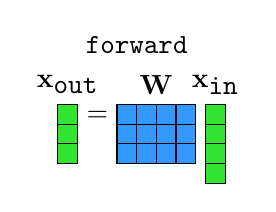
\begin{tikzpicture}
\draw[step=0.25cm,draw=black,fill=forwardpropcolor] (0,0) grid (0.25,-0.75) rectangle (0,0); \node at (0.125,0.25) {$\xout$};
\draw (0.5,-0.15) node {$=$};
\draw[step=0.25cm,draw=black,fill=param_color] (0.75,0) grid (1.75,-0.75) rectangle (0.75,0); \node at (1.25,0.25) {$\mathbf{W}$};
\draw[step=0.25cm,draw=black,fill=forwardpropcolor,shift={(0.125,0)}] (1.75,0) grid (2.0,-1.0) rectangle (1.75,0); \node at (2.0,0.25) {$\xin$};
\draw (1.0,0.75) node {\texttt{forward}};
\end{tikzpicture}
\end{minipage}
%
\begin{minipage}{0.33\linewidth}
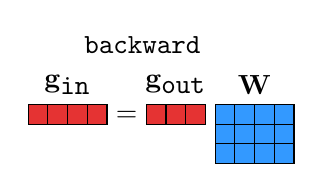
\begin{tikzpicture}
\draw[step=0.25cm,draw=black,fill=backwardpropcolor] (0,0) grid (1.0,-0.25) rectangle (0,0); \node at (0.5,0.25) {$\costgrad_{\texttt{in}}$};
\draw (1.25,-0.15) node {$=$};
\draw[step=0.25cm,draw=black,fill=backwardpropcolor] (1.5,0) grid (2.25,-0.25) rectangle (1.5,0); \node at (1.875,0.25) {$\costgrad_{\texttt{out}}$};
\draw[step=0.25cm,draw=black,fill=param_color,shift={(0.875,0)}] (1.5,0) grid (2.5,-0.75) rectangle (1.5,0); \node at (2.875,0.25) {$\mathbf{W}$};
\draw (1.45,0.75) node {\texttt{backward}};
\end{tikzpicture}
\end{minipage}
\end{figure}

Unlike the other equations, at first glance $\frac{\partial J}{\partial \mathbf{W}}$ does not seem to have a simple form. A naive approach would be to first build out the large sparse matrix $\localgrad^{\mathbf{W}}_{\texttt{out}}$ (which is $[M \times MN]$, with zeros wherever $i \neq k$ in $\localgrad^\mathbf{W}[i,jk]$), then do the matrix multiply $\costgrad_{\texttt{out}}\localgrad^{\mathbf{W}}_{\texttt{out}}$. We can avoid all those multiplications by zero by observing the following simplification:
%If we adopt the convention that Jacobians $\frac{\partial \mathbf{y}}{\partial \mathbf{x}}$ are written with $\partial \mathbf{y}_i$ indexed along the rows and $\partial \mathbf{x}_j$ indexed along the columns, 
%We can collate all the indices in Equations \ref{lingrad1} and \ref{lingrad3} into simple compact forms:
% \begin{align}
%     \frac{\partial \xout}{\partial \xin} &= \mathbf{W} & \quad\quad \triangleleft \quad [M \times N]\\
%     \frac{\partial \xout}{\partial \mathbf{b}} &= \mathbf{I} & \quad\quad \triangleleft \quad [M \times M]
% \end{align}
%The same doesn't work for $\frac{\partial \xout}{\mathbf{W}}$, since we have not defined a compact notation for gradients of a vector with respect to a matrix. We will set it aside for the moment.

% Now we can compute the gradients with respect to the loss via the chain rule, using Equations \ref{update_x} and \ref{update_theta}.
% \begin{align}
%     \frac{\partial \mathcal{L}}{\partial \xin} = \frac{\partial \mathcal{L}}{\partial \xout} \frac{\partial \xout}{\partial \xin} = \frac{\partial \mathcal{L}}{\partial \xout}\mathbf{W} & \quad\quad \triangleleft [1 \times M][M \times N] \rightarrow [1 \times N]\\
%     \frac{\partial \mathcal{L}}{\partial \mathbf{b}} = \frac{\partial \mathcal{L}}{\partial \xout} \frac{\partial \xout}{\partial \mathbf{b}} = \frac{\partial \mathcal{L}}{\partial \xout} \mathbf{I} & \quad\quad \triangleleft [1 \times M][M \times M] \rightarrow [1 \times M]
% \end{align}
\marginnote{In matrix equations, it's very useful to check that the dimensions all match up. To the right of each equation, we denote the dimensionality of the matrices in the product, where $\xin$ is M dimensions, $\xout$ is N dimensions, and the loss $J$ is always a scalar.}[3.2cm]

%We still need the gradient of the loss with respect to $\mathbf{W}$. First, we will write out the gradient with respect to each term $\mathbf{W}_{ij}$, then we will see that the update collapses to a compact form.
\begin{align}
    \frac{\partial J}{\partial \mathbf{W}[i,j]} 
        &= \frac{\partial J}{\partial \xout} \frac{\partial \xout}{\partial \mathbf{W}[i,j]} & \quad\quad \triangleleft [1 \times M][M \times 1] \rightarrow [1 \times 1]\\
        &= \frac{\partial J}{\partial \xout} [\frac{\partial \xout[1]}{\partial \mathbf{W}[i,j]}, \ldots ,\frac{\partial \xout[M]}{\partial \mathbf{W}[i,j]} ]^T\\
        &= \frac{\partial J}{\partial \xout} [\ldots , 0, \ldots , \frac{\partial \xout[i]}{\partial \mathbf{W}[i,j]}, \ldots, 0, \ldots ]^T\\
        &= \frac{\partial J}{\partial \xout} [\ldots , 0, \ldots , \xin_j, \ldots, 0, \ldots ]^T\\
        &= \frac{\partial J}{\partial \xout[i]}\xin[j] & \quad\quad \triangleleft [1 \times 1][1 \times 1] \rightarrow [1 \times 1]
\end{align}
Now we can just arrange all these scalar derivatives into the matrix for $\frac{\partial J}{\partial \mathbf{W}}$, and obtain the following:
\begin{align}
    \frac{\partial J}{\partial \mathbf{W}} & = 
        \begin{bmatrix}
            \frac{\partial J}{\partial \mathbf{W}[1,1]} & \ldots & \frac{\partial J}{\partial \mathbf{W}[N,1]} \\
            \vdots & \ddots & \vdots \\
            \frac{\partial J}{\partial \mathbf{W}[1,M]} & \ldots & \frac{\partial J}{\partial \mathbf{W}[N,M]} \\
        \end{bmatrix}\\
        & = 
        \begin{bmatrix}
            \frac{\partial J}{\partial \xout_1}\xin[1] & \ldots & \frac{\partial J}{\partial \xout[N]}\xin[1] \\
            \vdots & \ddots & \vdots \\
            \frac{\partial J}{\partial \xout[1]}\xin[M] & \ldots & \frac{\partial J}{\partial \xout[N]}\xin[M] \\
        \end{bmatrix}\\
        & = \xin \frac{\partial J}{\partial \xout}\\
        &= \xin \costgrad_{\texttt{out}}
\end{align}
So we see that in the end this gradient has the simple form of an outer product between two vectors, $\xin$ and $\costgrad_{\texttt{out}}$:  %Plugging these gradients into the parameter update rule we have:
% \begin{align}
%     \mathbf{W}^{t+1} &\leftarrow \mathbf{W}^t + \eta (\xin \frac{\partial \mathcal{L}}{\partial \xout})^T\\
%     \mathbf{b}^{t+1} &\leftarrow \mathbf{b}^t + \eta (\frac{\partial \mathcal{L}}{\partial \xout})^T
% \end{align}
% where we had to transpose $\frac{\partial \mathcal{L}}{\partial \xout}$ and $\xin \frac{\partial \mathcal{L}}{\partial \xout}$ so that the indices line up (remember how the shapes got transposed, by convention, in Equations \ref{backprop:scalar_vector_deriv} and  \ref{backprop:scalar_matrix_deriv}).

\begin{figure}[h]
\centering
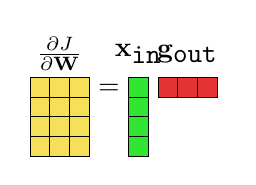
\begin{tikzpicture}
\draw[step=0.25cm,draw=black,fill=comp_graph_param_bcolor] (0,0) grid (0.75,-1.0) rectangle (0,0); \node at (0.375,0.3) {$\frac{\partial J}{\partial \mathbf{W}}$};
\draw (1.0,-0.15) node {$=$};
\draw[step=0.25cm,draw=black,fill=forwardpropcolor] (1.25,0) grid (1.5,-1.0) rectangle (1.25,0); \node at (1.375,0.3) {$\xin$};
\draw[step=0.25cm,draw=black,fill=backwardpropcolor,shift={(0.125,0)}] (1.5,0) grid (2.25,-0.25) rectangle (1.5,0); \node at (2,0.3) {$\costgrad_{\texttt{out}}$};
\end{tikzpicture}
\end{figure}

We can summarize all these operations in the following \texttt{forward} and \texttt{backward} diagram for linear layer:
\begin{figure}[h]
\centering
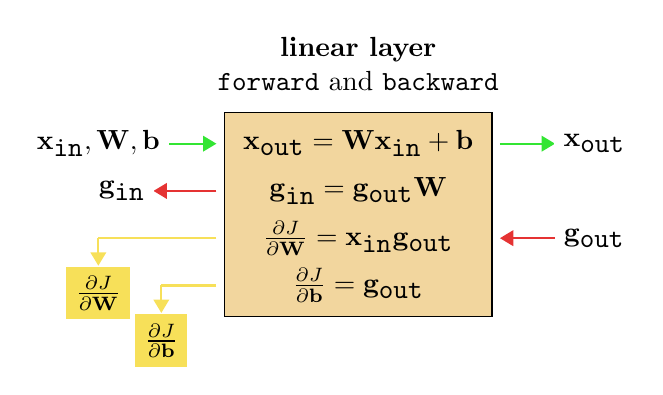
\begin{tikzpicture}%[>=spaced latex]
%
\def\layerwidth{2.0}
%
\draw [thick] [comp_graph_edge_forward] (0.4,0.6) -- (\layerwidth*0.6,0.6);
\draw [thick] [comp_graph_edge_backward] (\layerwidth*0.6,0) -- (0.4,0);
\draw [thick] [comp_graph_edge_backward_params] (-0.3,-0.6) -- (-0.3,-0.95);
\draw [thick] [color=backwardpropcolor_params] (\layerwidth*0.6,-0.6) -- (-0.3,-0.6);
\draw [thick] [comp_graph_edge_backward_params] (0.5,-1.2) -- (0.5,-1.55);
\draw [thick] [color=backwardpropcolor_params] (\layerwidth*0.6,-1.2) -- (0.5,-1.2);
\draw (\layerwidth*1.5,-0.3) node [fill=comp_graph_node_bcolor,draw, inner sep=2mm, minimum height=2.6cm, minimum width=3.4cm] {};
\draw (\layerwidth*1.5,1.8) node {\textbf{linear layer}};
\draw (\layerwidth*1.5,1.4) node {\texttt{forward} and \texttt{backward}};
\draw (\layerwidth*1.5,0.6) node  {$\xout = \mathbf{W}\xin + \mathbf{b}$};
\draw (\layerwidth*1.5,0) node  {$\costgrad_{\texttt{in}} = \costgrad_{\texttt{out}}\mathbf{W}$};
\draw (\layerwidth*1.5,-0.6) node  {$\frac{\partial J}{\partial \mathbf{W}} = \xin \costgrad_{\texttt{out}}$};
\draw (\layerwidth*1.5,-1.2) node  {$\frac{\partial J}{\partial \mathbf{b}} = \costgrad_{\texttt{out}}$};
\draw [thick] [comp_graph_edge_forward] (\layerwidth*2.4,0.6) -- (\layerwidth*2.75,0.6);
\draw [thick] [comp_graph_edge_backward] (\layerwidth*2.8,-0.6) -- (\layerwidth*2.4,-0.6);
%
\draw (-0.3,-1.3) node [fill=comp_graph_param_bcolor] {$\frac{\partial J}{\partial \mathbf{W}}$};
\draw (0.5,-1.9) node [fill=comp_graph_param_bcolor] {$\frac{\partial J}{\partial \mathbf{b}}$};
\draw (-0.3,0.6) node [fill=comp_graph_data_bcolor] {$\xin, \mathbf{W}, \mathbf{b}$};
\draw (0,0) node [fill=comp_graph_data_bcolor] {$\costgrad_{\texttt{in}}$};
\draw (\layerwidth*3,-0.6) node [fill=comp_graph_data_bcolor] {$\costgrad_{\texttt{out}}$};
\draw (\layerwidth*3,0.6) node [fill=comp_graph_data_bcolor] {$\xout$};
%
\end{tikzpicture}
\label{fig:backpropagation:linear_layer_backprop}
\end{figure}

%This may have looked a bit complicated, but it's completely mechanical, just a lot of bookkeeping of indices. In practice we rarely derive these updates by hand; instead we use programs to automatically compute them.

Notice that all these operations are simple expressions, mainly involving matrix multiplies. \texttt{Forward} and \texttt{backward} for a linear layer are also very easy to write in code, using any library that provides matrix multiplication (\texttt{matmul}) as a primitive. Here is Python code for this layer:
\begin{figure}[h]
\centering
\begin{minipage}{0.5\linewidth}
\begin{minted}[
fontsize=\fontsize{8.5}{9},
frame=single,
framesep=2.5pt,
baselinestretch=1.05,
]{python}

class linear():
    def __init__(self, W, b, lr):
        self.W = W
        self.b = b
        self.lr = lr # learning rate
        
    def forward(self, x_in):
        self.x_in = x_in
        return matmul(W,x)+b
    
    def backward(self,J_out):
        J_in = matmul(J_out,W)
        dJdW = matmul(self.x_in,J_out)
        dJdb = J_out
        return J_in, dJdW, dJdb
    
    def update(self, dJdW, dJdb):
        self.W -= self.lr*dJdW.transpose()
        self.b -= self.lr*dJdb
\end{minted}
\end{minipage}
\end{figure}

\subsection{Backprop for a pointwise nonlinearity}

Pointwise nonlinearities have very simple \texttt{backward} functions. Let a (parameterless) scalar nonlinearity be $h: \mathbb{R} \rightarrow \mathbb{R}$ with derivative function $h^{\prime}: \mathbb{R} \rightarrow \mathbb{R}$. Define a  pointwise layer using $h$ as $f(\xin) = [h(\xin_{0}), \ldots, h(\xin_{N})]^T$. Then we have
\begin{align}
    \localgrad^{\mathbf{x}} &= f^{\prime}(\xin) = \texttt{diag}([h^\prime(\xin_{1}), \ldots, h^\prime(\xin_{N})]^T) \triangleq \mathbf{H}^\prime
\end{align}
\marginnote{$\texttt{diag}$ is the operator that places a vector on the diagonal of a matrix, whose other entries are all zero.}[-0.4cm]
There are no parameters to update, so we just have to calculate $\costgrad_{\texttt{in}}$ in the \texttt{backward} operation, using Equation \ref{eqn:backpropagation:backward}:
\begin{align}
    \costgrad_{\texttt{in}} = \costgrad_{\texttt{out}}\mathbf{H}^\prime
\end{align}

As an example, for a \texttt{relu} layer we have:
\begin{align}
    h^\prime(x) = 
        \begin{cases}
            1 &\text{if} \quad x \geq 0\\
            0 &\text{otherwise}
        \end{cases}
\end{align}
As a matrix multiply, the \texttt{backward} operation looks like this:
\begin{figure}[h]
\centering
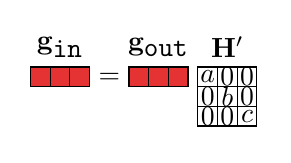
\begin{tikzpicture}
\draw[step=0.25cm,draw=black,fill=backwardpropcolor] (0.25,0) grid (1.0,-0.25) rectangle (0.25,0); \node at (0.625,0.25) {$\costgrad_{\texttt{in}}$};
\draw (1.25,-0.15) node {$=$};
\draw[step=0.25cm,draw=black,fill=backwardpropcolor] (1.5,0) grid (2.25,-0.25) rectangle (1.5,0); \node at (1.875,0.25) {$\costgrad_{\texttt{out}}$};
\draw[step=0.25cm,draw=black,fill=white,shift={(0.875,0)}] (1.5,0) grid (2.25,-0.75) rectangle (1.5,0); \node at (2.75,0.25) {$\mathbf{H}^{\prime}$};
\node at (2.5,-0.125) {$a$};
\node at (2.75,-0.125) {$0$};
\node at (3.0,-0.125) {$0$};
\node at (2.5,-0.375) {$0$};
\node at (2.75,-0.375) {$b$};
\node at (3.0,-0.375) {$0$};
\node at (2.5,-0.625) {$0$};
\node at (2.75,-0.625) {$0$};
\node at (3.0,-0.625) {$c$};
\end{tikzpicture}
\end{figure}

with $a = h^\prime(\xin_{1})$, $a = h^\prime(\xin_{2})$, and $a = h^\prime(\xin_{3})$. We can simplify this equation as follows:
\begin{align}
    \costgrad_{\texttt{in}}[i] = \costgrad_{\texttt{in}}[i]h^{\prime}(\xin[i]) \quad \forall i
\end{align}

The full set of operations for a pointwise layer then looks like this:
\begin{figure}[h]
\centering
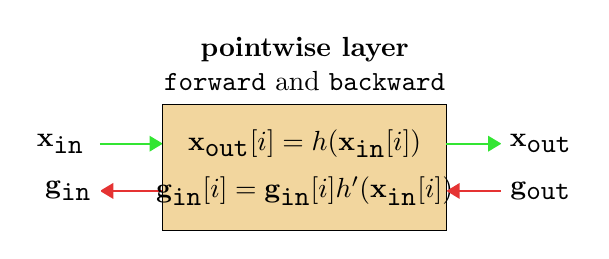
\begin{tikzpicture}%[>=spaced latex]
%
\def\layerwidth{2.0}
%
\draw [thick] [comp_graph_edge_forward] (0.4,0.6) -- (\layerwidth*0.6,0.6);
\draw [thick] [comp_graph_edge_backward] (\layerwidth*0.6,0) -- (0.4,0);
\draw (\layerwidth*1.5,0.3) node [fill=comp_graph_node_bcolor,draw, inner sep=2mm, minimum height=1.6cm, minimum width=3.6cm] {};
\draw (\layerwidth*1.5,1.8) node {\textbf{pointwise layer}};
\draw (\layerwidth*1.5,1.4) node {\texttt{forward} and \texttt{backward}};
\draw (\layerwidth*1.5,0.6) node  {$\xout[i] = h(\xin[i])$};
\draw (\layerwidth*1.5,0) node  {$\costgrad_{\texttt{in}}[i] = \costgrad_{\texttt{in}}[i]h^{\prime}(\xin[i])$};
\draw [thick] [comp_graph_edge_forward] (\layerwidth*2.4,0.6) -- (\layerwidth*2.75,0.6);
\draw [thick] [comp_graph_edge_backward] (\layerwidth*2.8,0) -- (\layerwidth*2.4,0);
%
\draw (-0.1,0.6) node [fill=comp_graph_data_bcolor] {$\xin$};
\draw (0,0) node [fill=comp_graph_data_bcolor] {$\costgrad_{\texttt{in}}$};
\draw (\layerwidth*3,0.0) node [fill=comp_graph_data_bcolor] {$\costgrad_{\texttt{out}}$};
\draw (\layerwidth*3,0.6) node [fill=comp_graph_data_bcolor] {$\xout$};
%
\end{tikzpicture}
\label{fig:backpropagation:pointwise_layer_backprop}
\end{figure}


\subsection{Backprop for loss layers}
The last layer we need to define for a complete MLP is the loss layer. As a simple example, we will derive backprop for an $L_2$ loss function: $\norm{\hat{\mathbf{y}} - \mathbf{y}}^2_2$, where $\hat{\mathbf{y}}$ is the output of the network (prediction) and $\mathbf{y}$ is the ground truth.

This layer has no parameters so we only need to derive Equation \ref{eqn:backpropagation:backward} for this layer:
\begin{align}
    \localgrad_{\out}^{\mathbf{x}} &= \frac{\partial \norm{\hat{\mathbf{y}} - \mathbf{y}}^2_2}{\partial \hat{\mathbf{y}}} = \hat{\mathbf{y}} - \mathbf{y} \quad\quad \triangleleft \quad [1 \times |\mathbf{y}|]\\
    \costgrad_{\texttt{in}} &= \costgrad_{\texttt{out}}(\hat{\mathbf{y}} - \mathbf{y}) = \hat{\mathbf{y}} - \mathbf{y}
\end{align}
Here we have made use of the fact that $\costgrad_{\texttt{out}} = \frac{\partial J}{\partial \xout} = \frac{\partial J}{\partial J} = 1$, since the output of the loss layer \textit{is} the cost $J$.

So, the backward signal sent by the $L_2$ loss layer is a row vector of per-dimension errors between the prediction and the target.

This completes our derivation of $\texttt{forward}$ and $\texttt{backward}$ for a $L_2$ loss layer:
\begin{figure}[h]
\centering
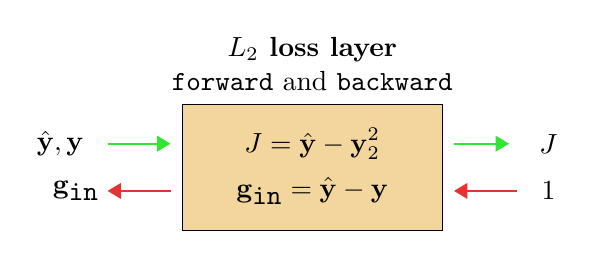
\begin{tikzpicture}%[>=spaced latex]
%
\def\layerwidth{2.0}
%
\draw [thick] [comp_graph_edge_forward] (0.4,0.6) -- (\layerwidth*0.6,0.6);
\draw [thick] [comp_graph_edge_backward] (\layerwidth*0.6,0) -- (0.4,0);
\draw (\layerwidth*1.5,0.3) node [fill=comp_graph_node_bcolor,draw, inner sep=2mm, minimum height=1.6cm, minimum width=3.3cm] {};
\draw (\layerwidth*1.5,1.8) node {\textbf{$L_2$ loss layer}};
\draw (\layerwidth*1.5,1.4) node {\texttt{forward} and \texttt{backward}};
\draw (\layerwidth*1.5,0.6) node  {$J = \norm{\hat{\mathbf{y}} - \mathbf{y}}^2_2$};
\draw (\layerwidth*1.5,0) node  {$\costgrad_{\texttt{in}} = \hat{\mathbf{y}} - \mathbf{y}$};
\draw [thick] [comp_graph_edge_forward] (\layerwidth*2.4,0.6) -- (\layerwidth*2.75,0.6);
\draw [thick] [comp_graph_edge_backward] (\layerwidth*2.8,0) -- (\layerwidth*2.4,0);
%
\draw (-0.2,0.6) node [fill=comp_graph_data_bcolor] {$\hat{\mathbf{y}}, \mathbf{y}$};
\draw (0,0) node [fill=comp_graph_data_bcolor] {$\costgrad_{\texttt{in}}$};
\draw (\layerwidth*3,0.0) node [fill=comp_graph_data_bcolor] {$1$};
\draw (\layerwidth*3,0.6) node [fill=comp_graph_data_bcolor] {$J$};
%
\end{tikzpicture}
\label{fig:backpropagation:L2_loss_layer_backprop}
\end{figure}

\subsection{Putting it all together: backprop through an MLP}
Let's see what happens when we put all these operations together in an MLP. We will start with the MLP in Figure \ref{fig:backpropagation:simple_MLP}. For simplicity, we will omit biases. Let $\mathbf{x}$ be 4-dimensional and $\mathbf{z}$ and $\mathbf{h}$ be 3-dimensional, and $\hat{\mathbf{y}}$ be 2-dimensional. Then the forward pass looks like this:
\begin{figure}[h]
\centering
\def\layerwidth{1.6}
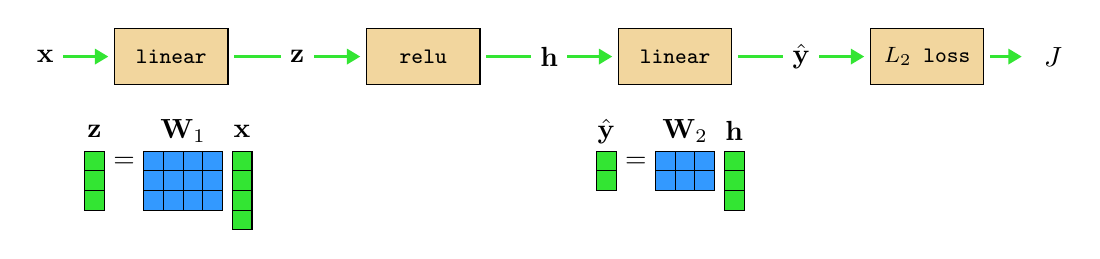
\begin{tikzpicture}[
cblock/.style={
draw,
fill=comp_graph_node_bcolor,
rectangle, 
inner sep=1.5mm,
minimum width=\layerwidth*0.9 cm,
minimum height=\layerwidth*0.5*0.9 cm,
font=\footnotesize}]
%
\def\offsety{-1.2}
\draw [thick] [comp_graph_edge_forward] (0,-\offsety) -- (\layerwidth*0.5,-\offsety);
%\draw (0,0) rectangle ++(1,1);
\draw (\layerwidth,-\offsety) node [cblock] {\texttt{linear}};
\draw [thick] [comp_graph_edge_forward] (\layerwidth*1.5,-\offsety) -- (\layerwidth*2.5,-\offsety);
\draw (\layerwidth*3,-\offsety) node [cblock] {\texttt{relu}};
\draw [thick] [comp_graph_edge_forward] (\layerwidth*3.5,-\offsety) -- (\layerwidth*4.5,-\offsety);
\draw (\layerwidth*5,-\offsety) node [cblock] {\texttt{linear}};
\draw [thick] [comp_graph_edge_forward] (\layerwidth*5.5,-\offsety) -- (\layerwidth*6.5,-\offsety);
\draw (\layerwidth*7,-\offsety) node [cblock] {\texttt{$L_2$ loss}};
\draw [thick] [comp_graph_edge_forward] (\layerwidth*7.5,-\offsety) -- (\layerwidth*7.75,-\offsety);
%
\draw (0,-\offsety) node [fill=comp_graph_data_bcolor] {$\mathbf{x}$};
\draw (\layerwidth*2,-\offsety) node [fill=comp_graph_data_bcolor] {$\mathbf{z}$};
\draw (\layerwidth*4,-\offsety) node [fill=comp_graph_data_bcolor] {$\mathbf{h}$};
\draw (\layerwidth*6,-\offsety) node [fill=comp_graph_data_bcolor] {$\hat{\mathbf{y}}$};
\draw (\layerwidth*8,-\offsety) node [fill=comp_graph_data_bcolor] {$J$};
%
% first linear layer matrix mult
\def\offsetx{0.5}
\draw[step=0.25cm,draw=black,fill=forwardpropcolor] (0+\offsetx,0) grid (0.25+\offsetx,-0.75) rectangle (0+\offsetx,0); \node at (0.125+\offsetx,0.25) {$\mathbf{z}$};
\draw (0.5+\offsetx,-0.15) node {$=$};
\draw[step=0.25cm,draw=black,fill=param_color] (0.75+\offsetx,0) grid (1.75+\offsetx,-0.75) rectangle (0.75+\offsetx,0); \node at (1.25+\offsetx,0.25) {$\mathbf{W}_1$};
\draw[step=0.25cm,draw=black,fill=forwardpropcolor,shift={(0.125,0)}] (1.75+\offsetx,0) grid (2.0+\offsetx,-1.0) rectangle (1.75+\offsetx,0); \node at (2.0+\offsetx,0.25) {$\mathbf{x}$};
%
% second linear layer matrix mult
\def\offsetx{7.0}
\draw[step=0.25cm,draw=black,fill=forwardpropcolor] (0+\offsetx,0) grid (0.25+\offsetx,-0.5) rectangle (0+\offsetx,0); \node at (0.125+\offsetx,0.25) {$\hat{\mathbf{y}}$};
\draw (0.5+\offsetx,-0.15) node {$=$};
\draw[step=0.25cm,draw=black,fill=param_color] (0.75+\offsetx,0) grid (1.5+\offsetx,-0.5) rectangle (0.75+\offsetx,0); \node at (1.125+\offsetx,0.25) {$\mathbf{W}_2$};
\draw[step=0.25cm,draw=black,fill=forwardpropcolor,shift={(0.125,0)}] (1.5+\offsetx,0) grid (1.75+\offsetx,-0.75) rectangle (1.5+\offsetx,0); \node at (1.75+\offsetx,0.25) {$\mathbf{h}$};
%
\end{tikzpicture}
\end{figure}

For the backward pass, we will here make a slight change in convention, which will clarify an interesting connection between the forward and backward directions. Rather than representing gradients $\costgrad$ as row vectors, we will transpose them and treat them as column vectors. The \texttt{backward} operation for transposed vectors follows from the matrix identity that $(\mathbf{A}\mathbf{B})^T = \mathbf{B}^T\mathbf{A}^T$:
\begin{align}
    \costgrad^T_{\texttt{in}} = (\costgrad_{\texttt{out}}\mathbf{W})^T = \mathbf{W}^T\costgrad^T_{\texttt{out}}
\end{align}

Now we will write the backward pass using these transposed $\localgrad$'s:
\begin{figure}[h]
\centering
\def\layerwidth{1.6}
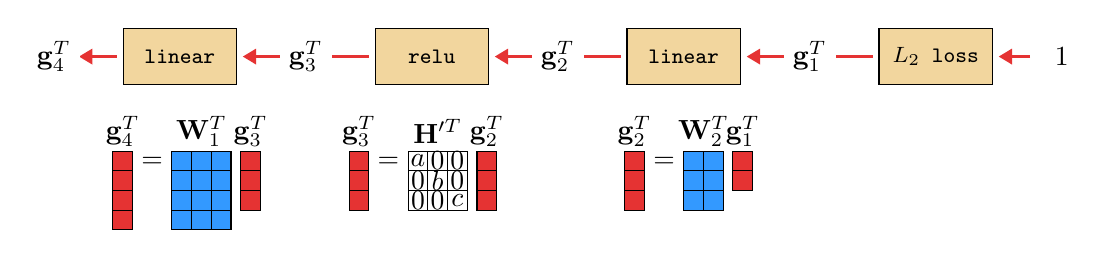
\begin{tikzpicture}[
cblock/.style={
draw,
fill=comp_graph_node_bcolor,
rectangle, 
inner sep=1.5mm,
minimum width=\layerwidth*0.9 cm,
minimum height=\layerwidth*0.5*0.9 cm,
font=\footnotesize}]
%
\def\offsety{-1.2}
\draw [thick] [comp_graph_edge_backward] (\layerwidth*0.5,-\offsety) -- (\layerwidth*0.2,-\offsety);
%\draw (0,0) rectangle ++(1,1);
\draw (\layerwidth,-\offsety) node [cblock] {\texttt{linear}};
\draw [thick] [comp_graph_edge_backward] (\layerwidth*2.5,-\offsety) -- (\layerwidth*1.5,-\offsety);
\draw (\layerwidth*3,-\offsety) node [cblock] {\texttt{relu}};
\draw [thick] [comp_graph_edge_backward] (\layerwidth*4.5,-\offsety) -- (\layerwidth*3.5,-\offsety);
\draw (\layerwidth*5,-\offsety) node [cblock] {\texttt{linear}};
\draw [thick] [comp_graph_edge_backward] (\layerwidth*6.5,-\offsety) -- (\layerwidth*5.5,-\offsety);
\draw (\layerwidth*7,-\offsety) node [cblock] {\texttt{$L_2$ loss}};
\draw [thick] [comp_graph_edge_backward] (\layerwidth*7.75,-\offsety) -- (\layerwidth*7.5,-\offsety);
%
\draw (0,-\offsety) node [fill=comp_graph_data_bcolor] {$\costgrad^T_4$};
\draw (\layerwidth*2,-\offsety) node [fill=comp_graph_data_bcolor] {$\costgrad^T_3$};
\draw (\layerwidth*4,-\offsety) node [fill=comp_graph_data_bcolor] {$\costgrad^T_2$};
\draw (\layerwidth*6,-\offsety) node [fill=comp_graph_data_bcolor] {$\costgrad^T_1$};
\draw (\layerwidth*8,-\offsety) node [fill=comp_graph_data_bcolor] {$1$};
%
% first linear layer matrix mult
\def\offsetx{0.75}
\draw[step=0.25cm,draw=black,fill=backwardpropcolor] (0+\offsetx,0) grid (0.25+\offsetx,-1) rectangle (0+\offsetx,0); \node at (0.125+\offsetx,0.25) {$\costgrad^T_4$};
\draw (0.5+\offsetx,-0.15) node {$=$};
\draw[step=0.25cm,draw=black,fill=param_color] (0.75+\offsetx,0) grid (1.5+\offsetx,-1) rectangle (0.75+\offsetx,0); \node at (1.125+\offsetx,0.25) {$\mathbf{W}^T_1$};
\draw[step=0.25cm,draw=black,fill=backwardpropcolor,shift={(0.125,0)}] (1.5+\offsetx,0) grid (1.75+\offsetx,-0.75) rectangle (1.5+\offsetx,0); \node at (1.75+\offsetx,0.25) {$\costgrad^T_3$};
%
% relu
\def\offsetx{3.75}
\draw[step=0.25cm,draw=black,fill=backwardpropcolor] (0+\offsetx,0) grid (0.25+\offsetx,-0.75) rectangle (0+\offsetx,0); \node at (0.125+\offsetx,0.25) {$\costgrad^T_3$};
\draw (0.5+\offsetx,-0.15) node {$=$};
\draw[step=0.25cm,draw=black,fill=white] (0.75+\offsetx,0) grid (1.5+\offsetx,-0.75) rectangle (0.75+\offsetx,0); \node at (1.125+\offsetx,0.25) {$\mathbf{H}^{\prime T}$};
\draw[step=0.25cm,draw=black,fill=backwardpropcolor,shift={(0.125,0)}] (1.5+\offsetx,0) grid (1.75+\offsetx,-0.75) rectangle (1.5+\offsetx,0); \node at (1.75+\offsetx,0.25) {$\costgrad^T_2$};
%
\node at (0.75+0.125+\offsetx,-0.125) {$a$};
\node at (1.0+0.125+\offsetx,-0.125) {$0$};
\node at (1.25+0.125+\offsetx,-0.125) {$0$};
\node at (0.75+0.125+\offsetx,-0.375) {$0$};
\node at (1.0+0.125+\offsetx,-0.375) {$b$};
\node at (1.25+0.125+\offsetx,-0.375) {$0$};
\node at (0.75+0.125+\offsetx,-0.625) {$0$};
\node at (1.0+0.125+\offsetx,-0.625) {$0$};
\node at (1.25+0.125+\offsetx,-0.625) {$c$};
%
% second linear layer matrix mult
\def\offsetx{7.25}
\draw[step=0.25cm,draw=black,fill=backwardpropcolor] (0+\offsetx,0) grid (0.25+\offsetx,-0.75) rectangle (0+\offsetx,0); \node at (0.125+\offsetx,0.25) {$\costgrad^T_2$};
\draw (0.5+\offsetx,-0.15) node {$=$};
\draw[step=0.25cm,draw=black,fill=param_color] (0.75+\offsetx,0) grid (1.25+\offsetx,-0.75) rectangle (0.75+\offsetx,0); \node at (1+\offsetx,0.25) {$\mathbf{W}^T_2$};
\draw[step=0.25cm,draw=black,fill=backwardpropcolor,shift={(0.125,0)}] (1.25+\offsetx,0) grid (1.5+\offsetx,-0.5) rectangle (1.25+\offsetx,0); \node at (1.5+\offsetx,0.25) {$\costgrad^T_1$};
%
\end{tikzpicture}
\end{figure}

This reveals an interesting connection between \texttt{forward} and \texttt{backward} for linear layers: \texttt{backward} for a linear layer is the same operation as \texttt{foward}, just with the weights transposed! We have omitted the bias terms here, but recall from Equation \ref{eqn:backpropagation:linear_backward_costgrad} that the backward pass to the activations ignores biases anyway.

In contrast, the \texttt{relu} layer is not a \texttt{relu} on the backward pass. Instead, it becomes a sort of ``gating" matrix, parameterized by functions of the activations from the forward pass ($a$, $b$, and $c$). This matrix is all zeros except for ones on the diagonal where the activation was non-negative. This layer acts to mask out gradients for variables on the negative side of the $\texttt{relu}$. Notice that this operation is a matrix multiply -- in fact, \textit{all} \texttt{backward} operations are matrix multiplies, no matter what the \texttt{forward} operation might be. You can observe this in Algorithm \ref{alg:backpropagation:backprop_for_chains} -- in fact, all \texttt{backward} operations are linear functions of $\costgrad_L$. This is an amazing fact that might seem surprising at first, but it follows straight from the definition of a gradient as the hyperplane that lies tangent to a cost function at a given point. So, if we fix the operating point, $\{\mathbf{x}_0, \theta\}$, then the description of the gradient must be the description of a hyperplane, i.e. a linear function.


\section{Backprop through DAGs: branch and merge}

So far we have only seen chain-like graphs, --[]--[]--[]$\rightarrow$. Can backprop handle other graphs? It turns out the answer is \textit{yes}. Presently we will consider {\bf directed acyclic graphs}, or {\bf DAGs}. In Chapter \ref{chapter:recurrent_neural_nets}, we will see that neural nets can also include cycles and still be trained with variants of backprop (e.g., backprop through time).

In a DAG, nodes can have multiple inputs and multiple outputs. In fact, we have already seen several examples of such nodes in the preceding sections. For example, a linear layer can be thought of as having two inputs, $\xin$ and $\theta$, and one output $\xout$; or it can be thought of as having $N = |\xin| + |\theta|$ inputs and $M = |\xout|$ outputs, if we count up each dimension of the input and output vectors. So we have already seen DAG computation graphs.

However, to work with general DAGs, it helps to introduce two new special modules, which act to construct the topology of the graph. We will call these special operators \texttt{branch} and \texttt{merge}. %\texttt{Branch} takes data and makes two copies of it, sent to two different subsequent modules. \texttt{Merge} takes two input data vectors and concatenates them into a single output vector. 
\begin{figure}[h]
    \centering
    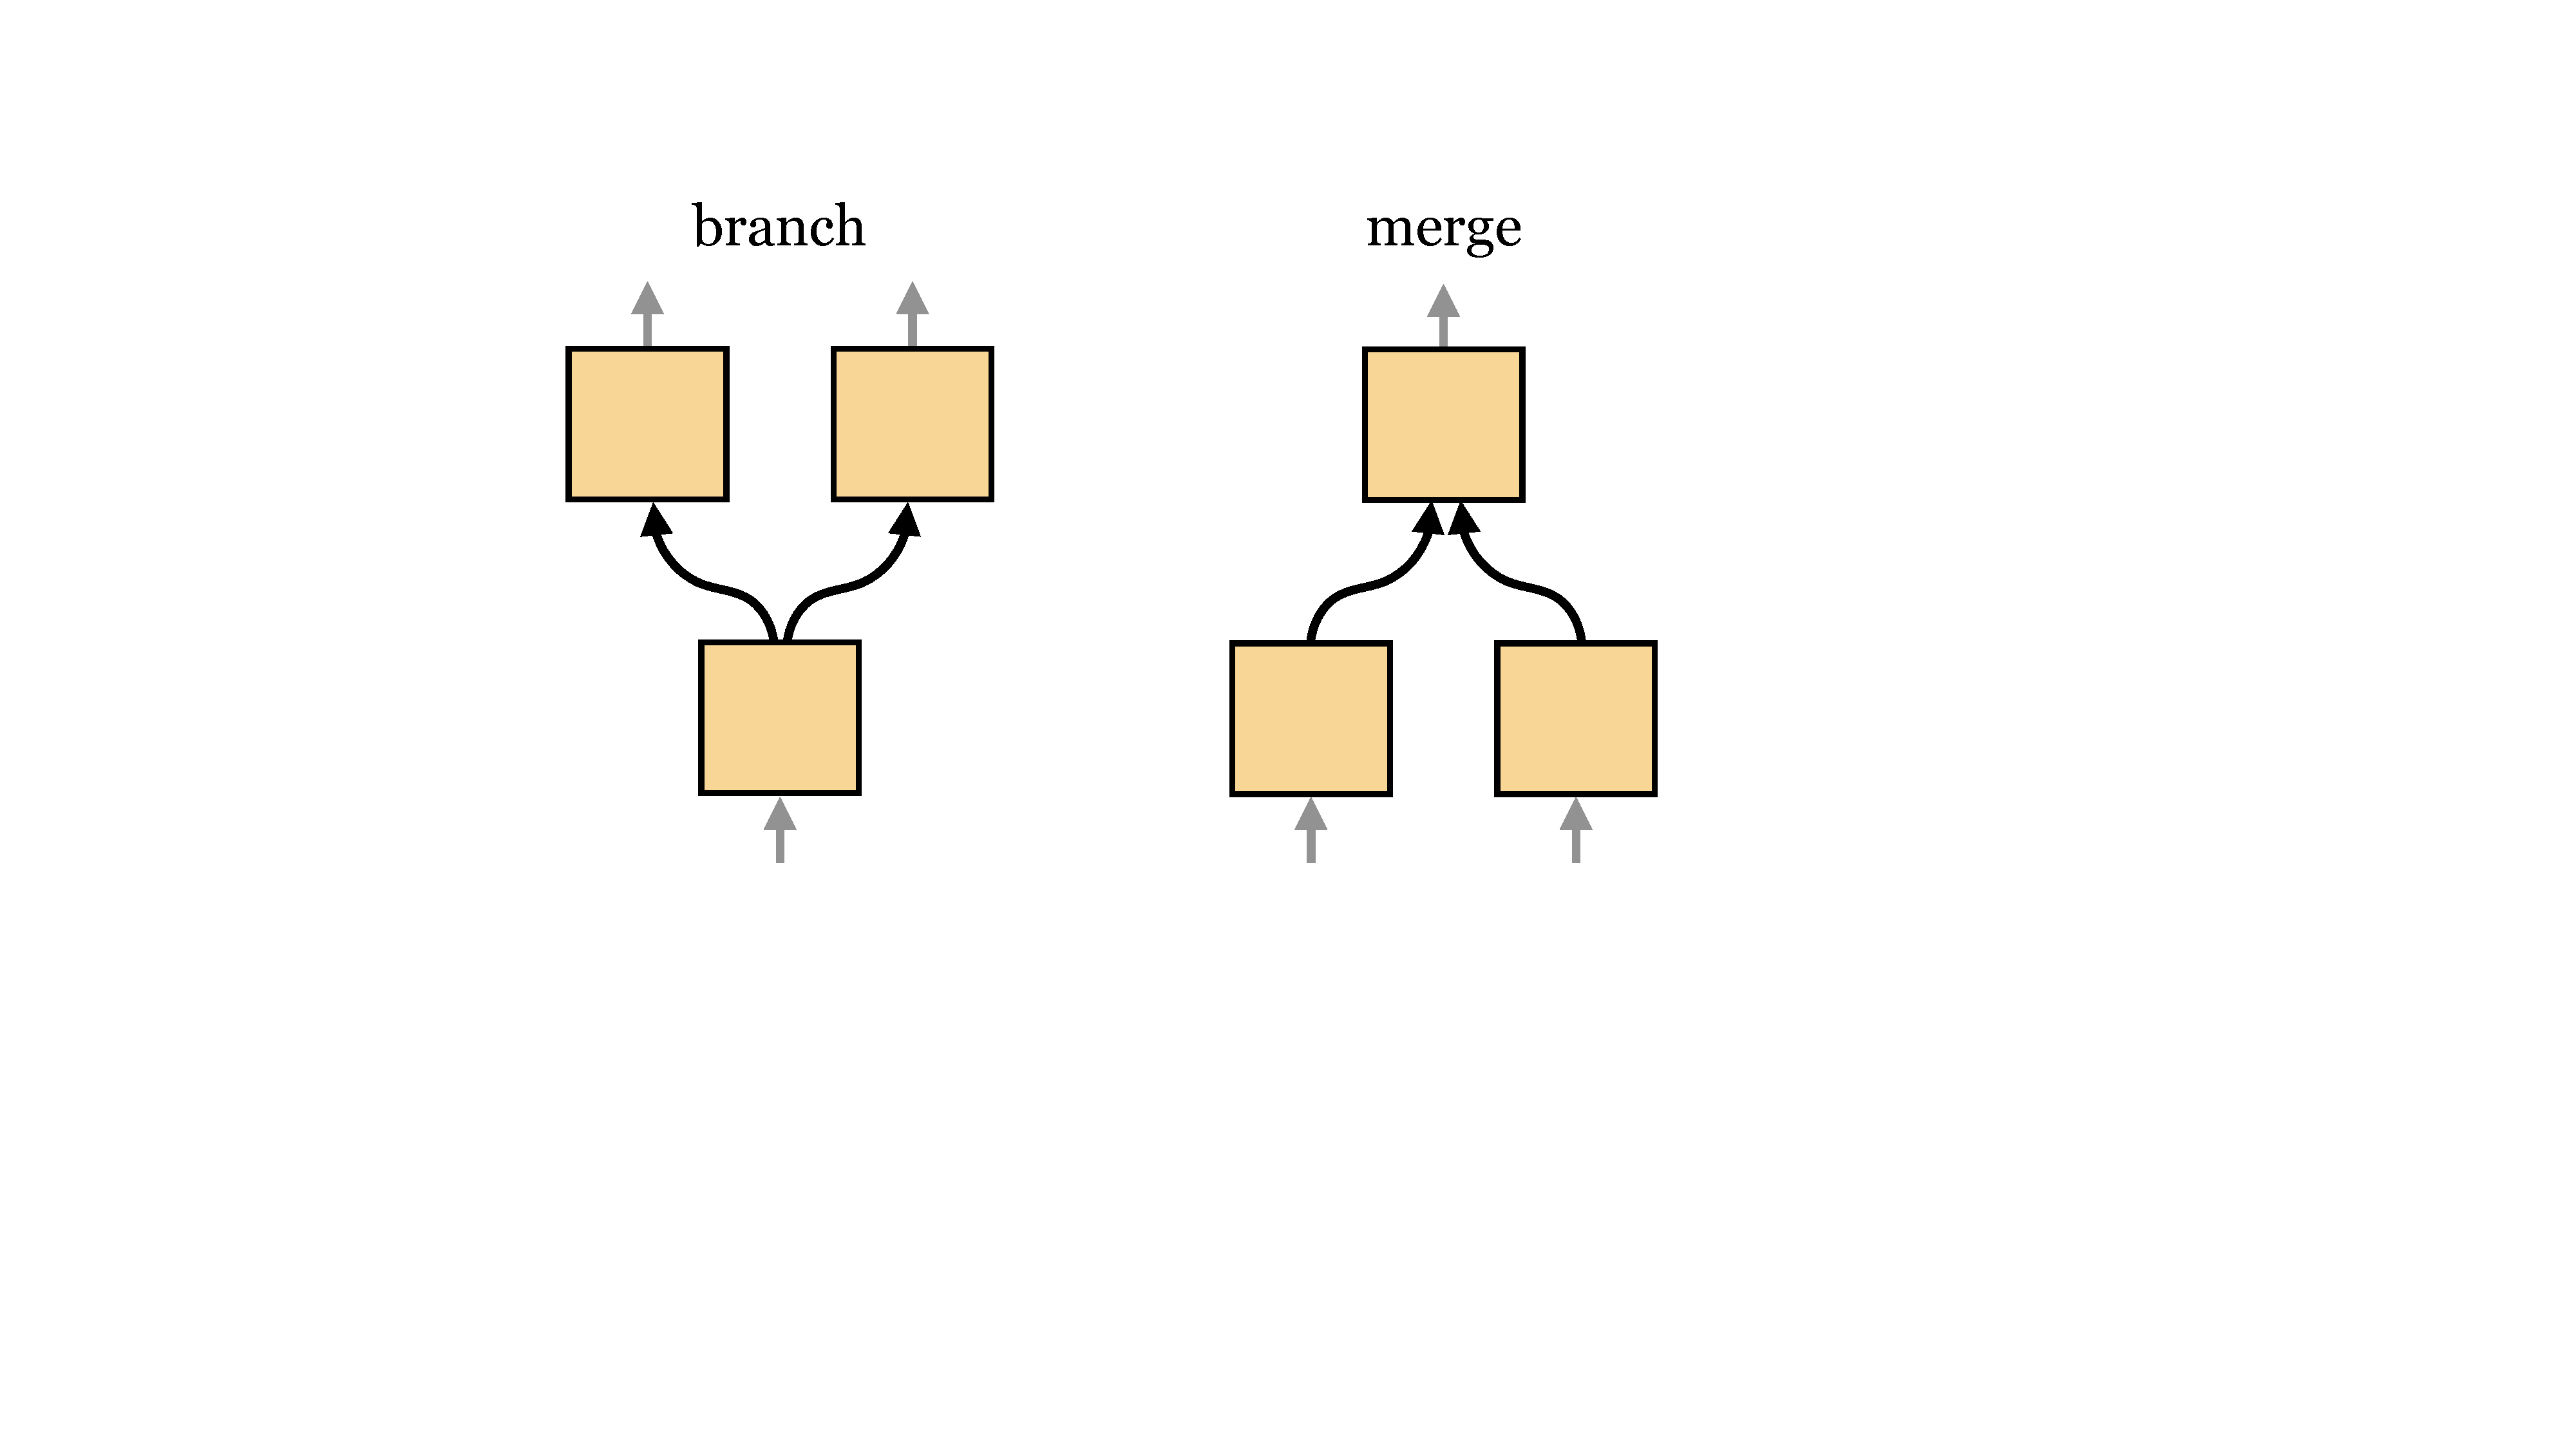
\includegraphics[width=0.42\linewidth]{./figures/backpropagation/branch_merge.pdf}
    \label{fig:backprop_branch_merge}
\end{figure}

\begin{align}
    \texttt{merge}(\mathbf{x}^a, \mathbf{x}^b, \ldots) &= [\mathbf{x}^a, \mathbf{x}^b, \ldots] \equiv \mathbf{x}^{\texttt{merged}}\\
    \texttt{branch}(\mathbf{x}) &= [\mathbf{x}, \mathbf{x}, \ldots] \equiv [\mathbf{x}^a, \mathbf{x}^b, \ldots]
\end{align}
\marginnote{What if $\mathbf{x}^a$ and $\mathbf{x}^b$ are tensors, or other objects, with different shapes? Can we still concatenate them? The answer is yes. The shape of the data tensor has no impact on the math. We pick the shape just as a notational convenience, e.g., it's natural to think about images as 2D arrays.}[-0.8cm]
$\texttt{merge}$ takes multiple inputs and concatenates them. This results in a new multidimensional variable. The backward pass equation is trivial. To compute the gradient with respect to $\mathbf{x}^{a}$ (and likewise for $\mathbf{x}^b$, $\mathbf{x}^c$, etc), we have
\begin{align}
    \frac{\partial J}{\partial \mathbf{x}^{a}} &= \frac{\partial J}{\partial \mathbf{x}^{\texttt{merged}}} \frac{\partial \mathbf{x}^{\texttt{merged}}}{\partial \mathbf{x}^{a}} = \frac{\partial J}{\partial \mathbf{x}} \frac{\partial \texttt{merge}}{\partial \mathbf{x}^{a}}\\
    &= \frac{\partial J}{\partial \mathbf{x}^{\texttt{merged}}} [\frac{\partial \mathbf{x}^{1}}{\partial \mathbf{x}^{i}}, \ldots, \frac{\partial \mathbf{x}^{i}}{\partial \mathbf{x}^{i}}, \ldots, \frac{\partial \mathbf{x}^{N}}{\partial \mathbf{x}^{i}}]^T\\
    &= \frac{\partial J}{\partial \mathbf{x}^{\texttt{merged}}} [0, \ldots, 1, \ldots, 0]^T
\end{align}
That is, we just pick out the i-th block of the $\frac{\partial J}{\partial \mathbf{x}^{\texttt{merged}}}$ Jacobian matrix. There is really nothing new here. We already defined backprop for multidimensional variables above, and $\texttt{merge}$ is just an explicit way of constructing multidimensional variables.

%We already defined backprop for multidimensional inputs, and nothing is different here. The gradients propagated backwards are $\frac{\partial J}{\partial \mathbf{x}^{\prime}}$.

\texttt{branch} is only slightly more complicated. In branching, we send \textit{copies} of the same output to multiple downstream nodes. Therefore, we have multiple gradients coming back to the $\texttt{branch}$ module, each from different downstream paths. So the inputs to this module on the backward pass are $\frac{\partial J}{\partial \mathbf{x}^{a}}, \frac{\partial J}{\partial \mathbf{x}^{b}}, \ldots$, which we can write as the Jacobian matrix $\frac{\partial J}{\partial [\mathbf{x}^a, \mathbf{x}^b, \ldots]} = [\frac{\partial J}{\partial \mathbf{x}^{a}}, \frac{\partial J}{\partial \mathbf{x}^{b}}, \ldots]$.  Let's compute the backwards pass output:
\begin{align}
    \frac{\partial J}{\partial \mathbf{x}} &= \frac{\partial J}{\partial [\mathbf{x}^a, \mathbf{x}^b, \ldots]} \frac{\partial [\mathbf{x}^a, \mathbf{x}^b, \ldots]}{\partial \mathbf{x}} = \frac{\partial J}{\partial [\mathbf{x}^a, \mathbf{x}^b, \ldots]} \frac{\partial \texttt{branch}}{\partial \mathbf{x}}\\
    &= [\frac{\partial J}{\partial \mathbf{x}^{a}}, \frac{\partial J}{\partial \mathbf{x}^{b}}, \ldots][1, 1, \ldots]^T\\
    &= \sum_{i} \frac{\partial J}{\partial \mathbf{x}^{i}}
\end{align}
So, branching just sums all the gradients passed backwards to it.
%Suppose our output is $\mathbf{x}^{l+1}$. Then, during backprop, we have multiple different versions of $\partial L \partial x$ being propagated back. How should resolve all these different versions? Consider the simple case where we have two output branches. 

Both $\texttt{merge}$ and $\texttt{branch}$ have no parameters, so there is no parameter gradient to define. Thus, we have fully specified the forward and backward behavior of these layers. 

These diagrams summarize the behavior:
\begin{figure}[h]
    \centering
    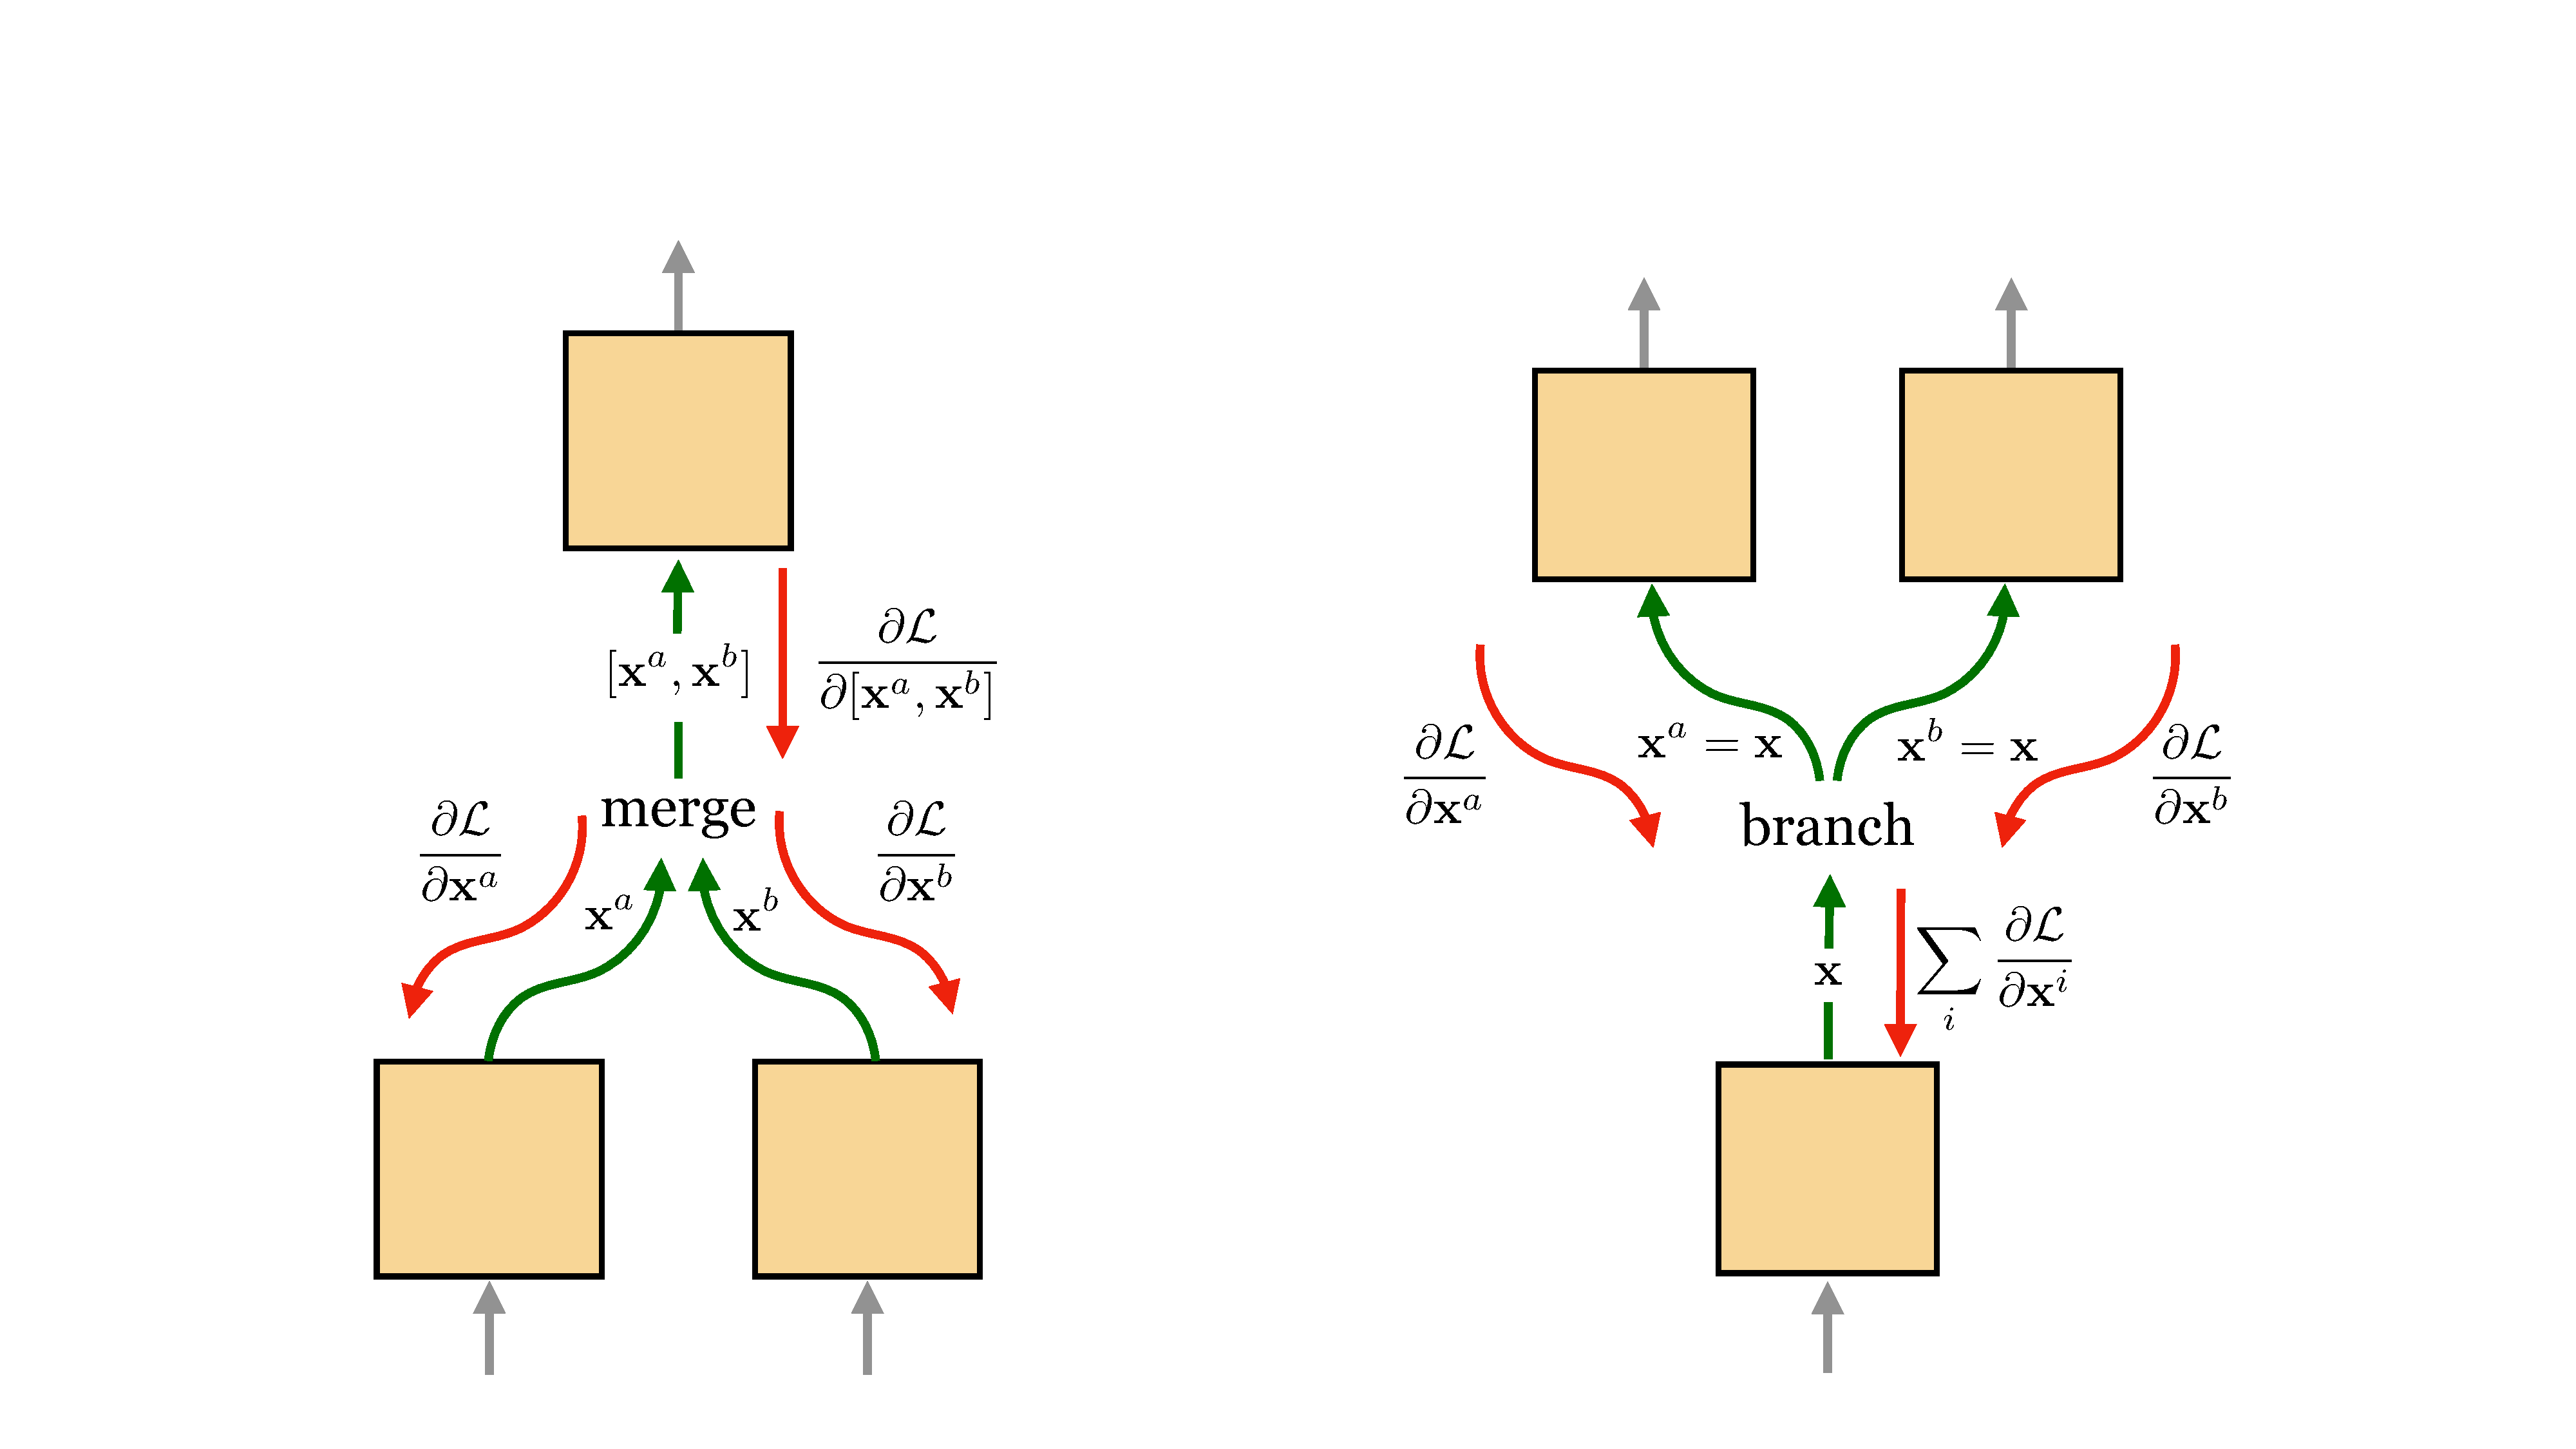
\includegraphics[width=0.75\linewidth]{./figures/backpropagation/branch_merge_gradient_diagrams.pdf}
    \label{fig:backprop_branch_merge_gradient_diagrams}
\end{figure}


\section{Computation graphs}
Now, we can constuct any directed acyclical \textbf{computation graph} (DAG) by simply inserting $\texttt{merge}$ or $\texttt{branch}$ layers wherever we want a node to have multiple inputs, or, respectively, multiple outputs.
\begin{figure}[h]
    \centering
    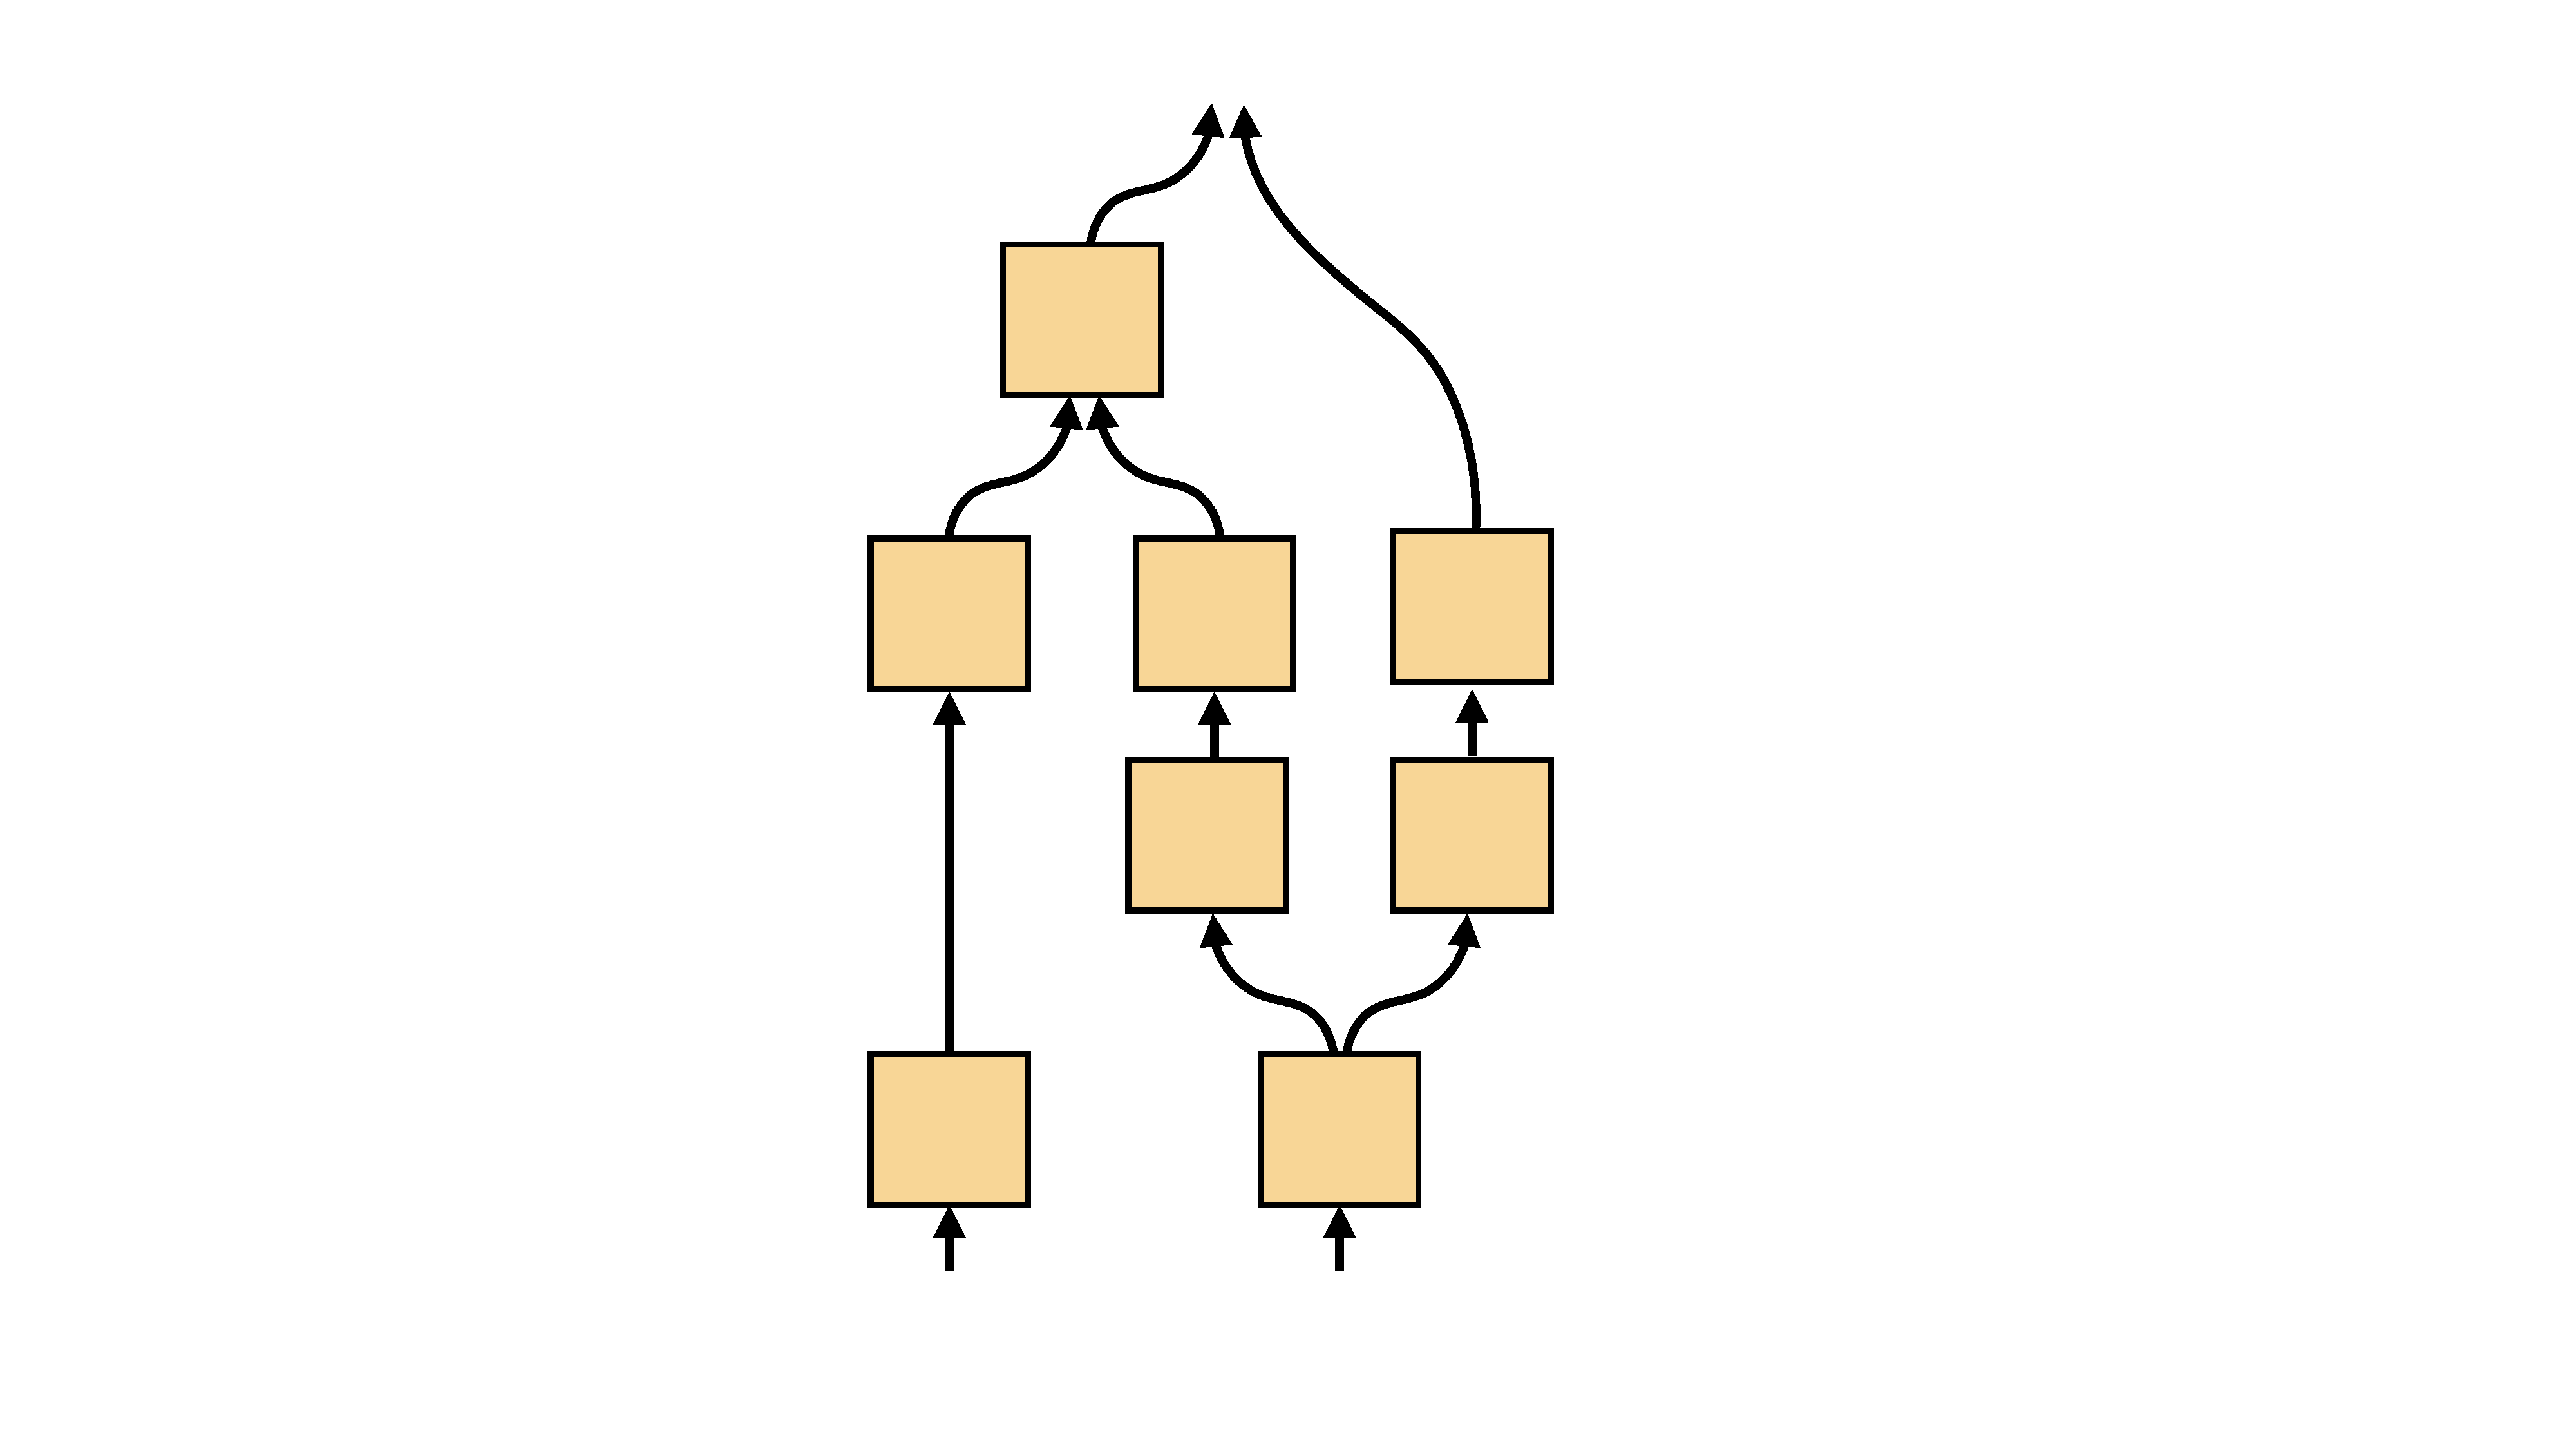
\includegraphics[width=0.16\linewidth]{./figures/backpropagation/DAG.pdf}
    \label{fig:backprop_DAG}
\end{figure}
\marginnote{An example of a DAG computation graph that we can construct, and do backprop through, with the tools defined above.}[1.6cm]

Given a differentiable computation graph, we can optimize any node or edge in the graph w.r.t. any other (scalar) node in the graph. For example, suppose we want to optimize some the value of some cost function (a scalar) indicated as the red node in the computation graph below. Using backprop, we can find and descend the gradient w.r.t. either a mapping at the top of the computation graph (yellow edge), or a w.r.t. some inputs at the bottom (yellow outlined node) or any other edge or node in this graph:
\begin{figure}[h]
    \centering
    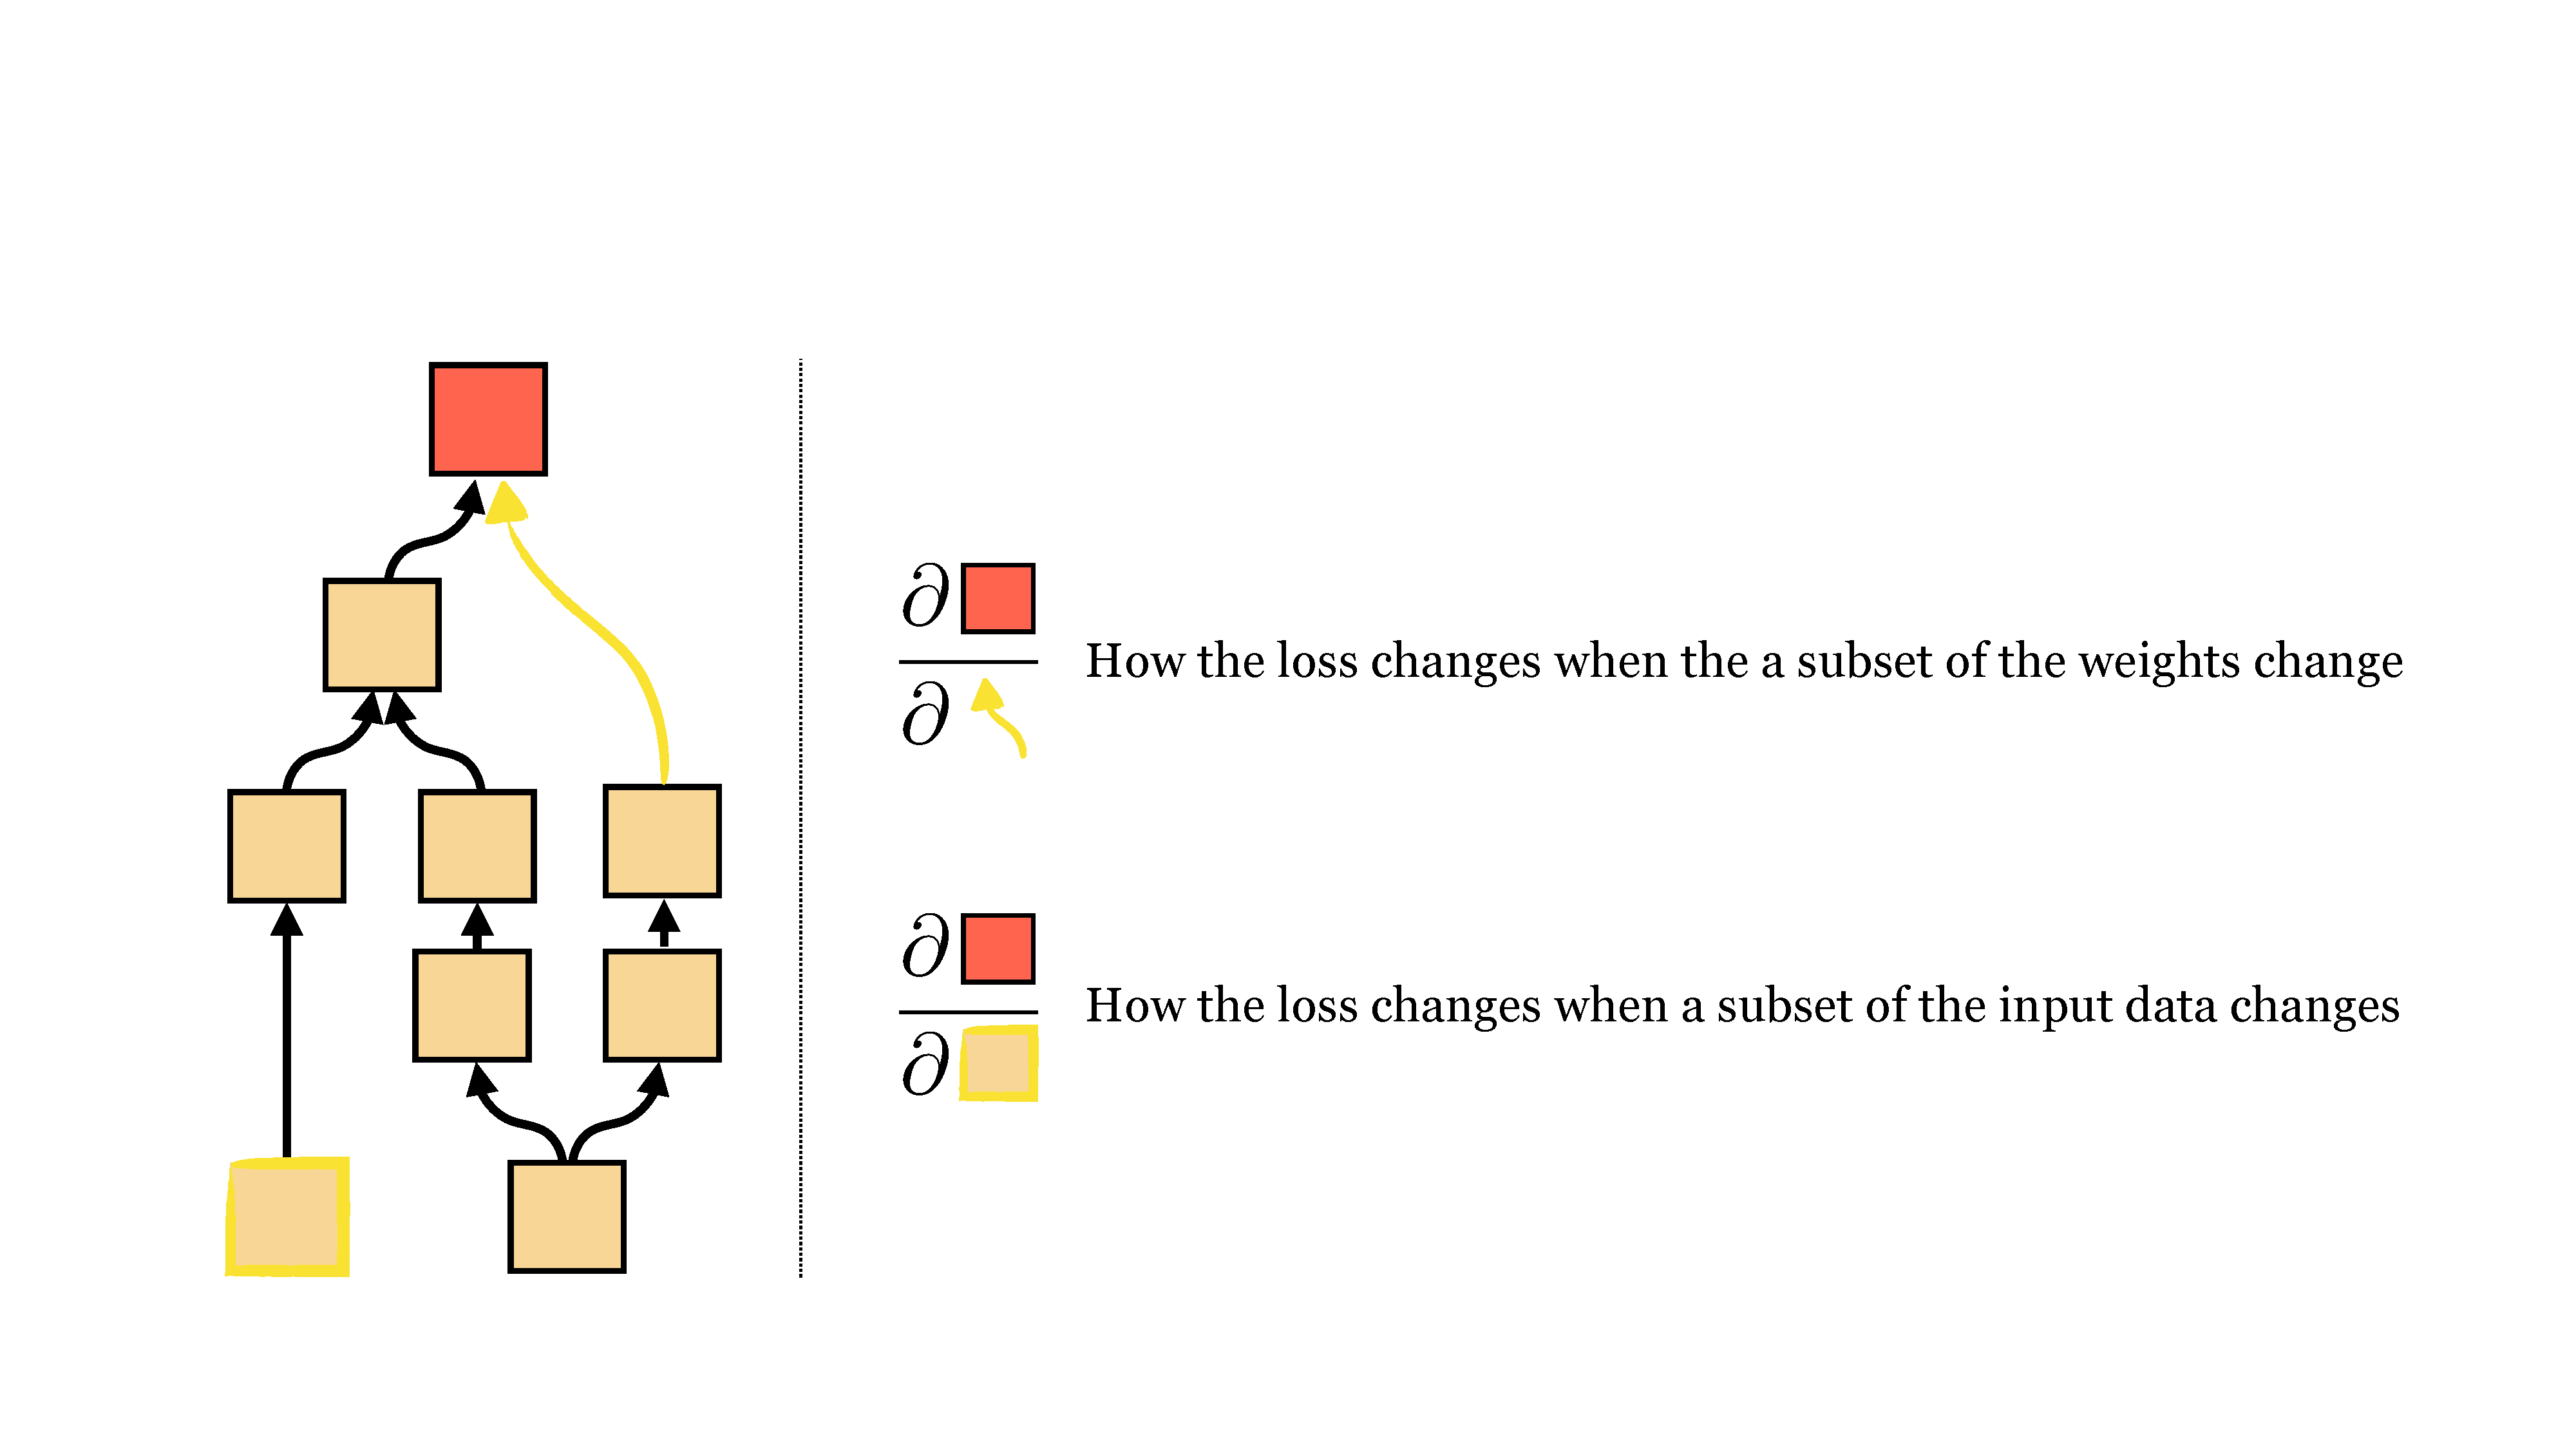
\includegraphics[width=0.9\linewidth]{./figures/backpropagation/computation_graph_opt.pdf}
    \label{fig:computation_graph_opt}
\end{figure}


\section{Parameter sharing}

Parameter sharing consists of a single parameter being sent as input to multiple different layers. We can consider this as a branching operation. Then, from the previous section, it is clear that gradients summate for shared parameters.

\section{Backprop to the data}

Backprop does not distinguish between parameters and data — it treats both as generic inputs to parameterless modules. Therefore, we can use backprop to optimize data inputs to the graph just like we can use backprop to optimize parameter inputs to the graph.

This can be useful for lots of different applications. One example is visualizing the input image that most activates a given neuron in a neural net. Here is what that looks like:

